%!TEX root = index.tex

% 1. Get familiar with air traffic, air space, and procedures related to operations in a terminal area.
% 2. Design general architecture of a simulated air traffic controller behavior model that works in a terminal area.
% 3. Implement general configurable air traffic controller model in the AgentFly system.
% 4. Implement specific air traffic controller model for selected airport and study influence of the behavior to an air traffic.

\documentclass[11pt,oneside,a4paper]{book}
%%%%\documentclass[11pt,twoside,a4paper]{book}   %%%%%%%%%%%%%%%%%%%%%%%%%%%%%%%%%%%%%%%%%%%%%%%%%%%%%%%%%%%%%%%%%%%%%%%%%%%%%%%%%

\usepackage[czech, english]{babel}
\usepackage[OT1]{fontenc} %[IL2] [T1] [OT1]
\usepackage[utf8]{inputenc}
\usepackage{lmodern}
\usepackage{graphicx}
\usepackage{color}
\usepackage{k336_thesis_macros}
%\usepackage{indentfirst} %1. odstavec jako v cestine.

\newcommand\TypeOfWork{Master's Thesis}
\newcommand\StudProgram{Open Informatics}
\newcommand\StudBranch{Software Engineering}
\newcommand\WorkTitle{Air Traffic Control Simulation in Terminal Area}
\newcommand\FirstandFamilyName{Bc. Jan Straka}
\newcommand\Supervisor{Mgr. Přemysl Volf, Ph.D}
\newcommand\Department{Department of Computer Science}
\newcommand\Faculty{Faculty of Electrical Engineering}
\newcommand\University{Czech Technical University in Prague}
\newcommand\labelSupervisor{Supervisor}
\newcommand\labelStudProgram{Study Programme} 
\newcommand\labelStudBranch{Field of Study}
\newcommand{\red}[1] {\textcolor{red}{#1}}

\usepackage[
pdftitle={\WorkTitle},
pdfauthor={\FirstandFamilyName},
bookmarks=true,
colorlinks=true,
breaklinks=true,
urlcolor=red,
citecolor=blue,
linkcolor=blue,
unicode=true,
]{hyperref}

\begin{document}
\selectlanguage{english} 

\coverpagestarts

% \acknowledgements
% \noindent
% Zde můžete napsat své poděkování, pokud chcete a máte komu děkovat.


% \declaration{In Prague on January 5, 2015}

 
% \abstractpage
% Translation of Czech abstract into English.
% \vglue60mm
% \noindent{\Huge \textbf{Abstrakt}}
% \vskip 2.75\baselineskip
% \noindent
% Abstrakt práce by měl velmi stručně vystihovat její podstatu. Tedy čím se práce zabývá a co je jejím výsledkem/přínosem.
% \noindent
% Očekávají se cca 1 -- 2 odstavce, maximálně půl stránky.


\tableofcontents
% \listoffigures
% \listoftables


\mainbodystarts
\normalfont
\parskip=0.2\baselineskip plus 0.2\baselineskip minus 0.1\baselineskip

%!TEX root = index.tex
\chapter{Introduction}

\section{Motivation – Why is Air Traffic Simulation needed?}
\section{Thesis goals}
%plane aircraft airplane interchangably
%!TEX root = index.tex
\chapter{State of the art}
\section{Definitions}

Air Traffic Control service (ATC) can be devided into: area control service (ACC), approach control service (APP) and aerodrome control service (TWR) \cite[Chapter 1]{doc4444} The main objective is to prevent collisions between aircraft in air or on land and to expedite the flow of air traffic. \cite[Chapter 2.2]{annex11}
The airspace in which ATC service is provided can be divided into Control area (CTA), Control Zones (CTR) and Controlled aerodromes (TWR). Control area contains airways, terminal control areas and other airspace. It extends upwards from specified altitude. Within CTA, terminal control areas (TMA) are established to help in arrival and departure at some airports.
Control zones are normally situated below CTA and encompass airspace used by flights arriving at and departing from aerodromes. The diameter of CTR is at least 5NM in direction from which airplanes approach. CTR extends from the ground at least to the lower limit of CTA, but may extend further. CTR may include several aerodromes situated close together. \cite[Chapter 2.10]{annex11}

\begin{figure}[h]
    \centering
    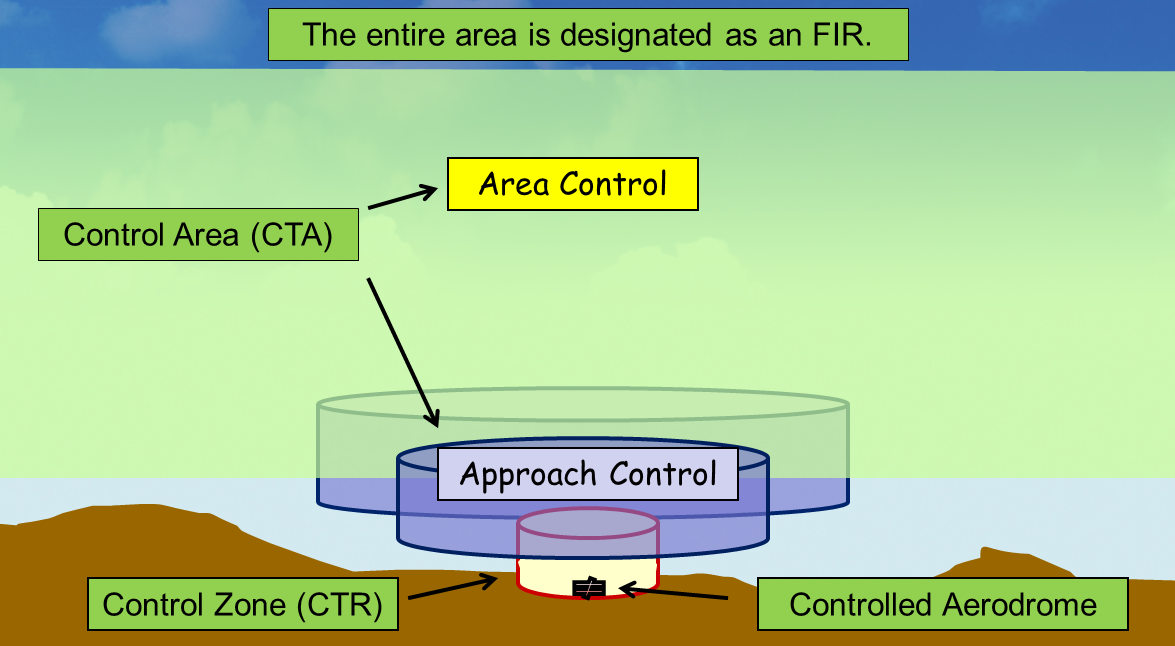
\includegraphics[width=0.8\textwidth]{figures/airspace.png}
    \caption{Airspace - \textcolor{red}{z prezentace 2011 ATM Lesson Plans/ATM 1-1 General Air Traffic Services podle \cite[Chapter 2.5]{annex11} - překreslit!}}
    \label{fig:airspace}
\end{figure}

\begin{figure}[h]
    \centering
    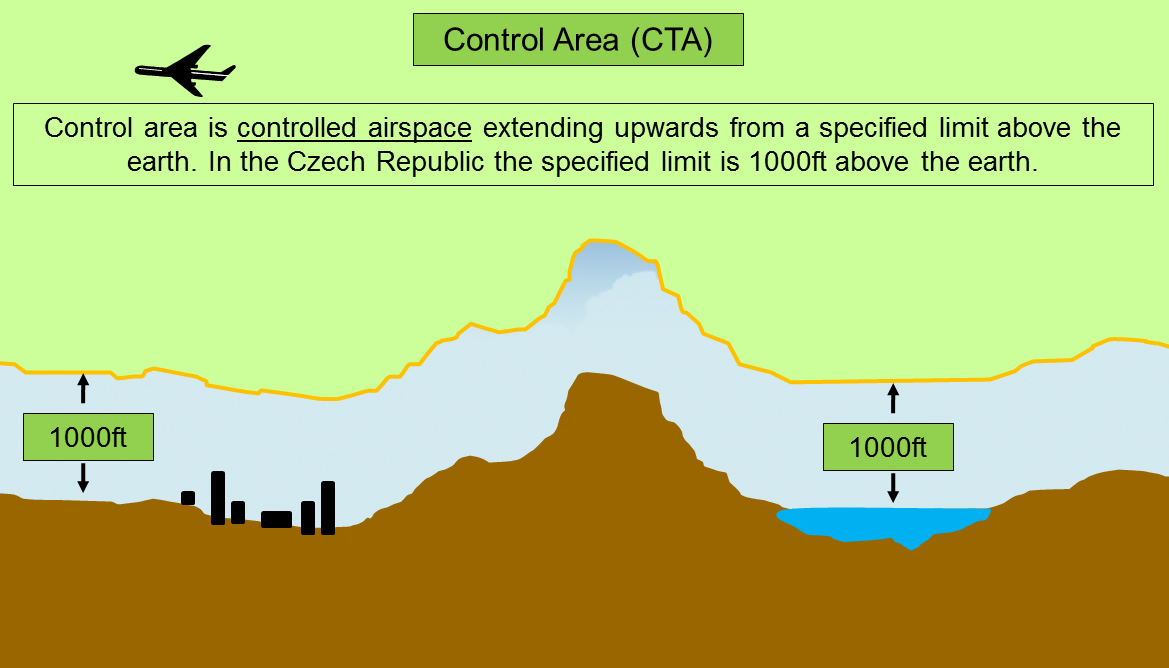
\includegraphics[width=0.8\textwidth]{figures/cta.png}
    \caption{CTA - \textcolor{red}{z prezentace 2011 ATM Lesson Plans/ATM 1-1 General Air Traffic Services podle \cite[Chapter 2.10]{annex11} - překreslit!}}
    \label{fig:cta}
\end{figure}

\begin{figure}[h]
    \centering
    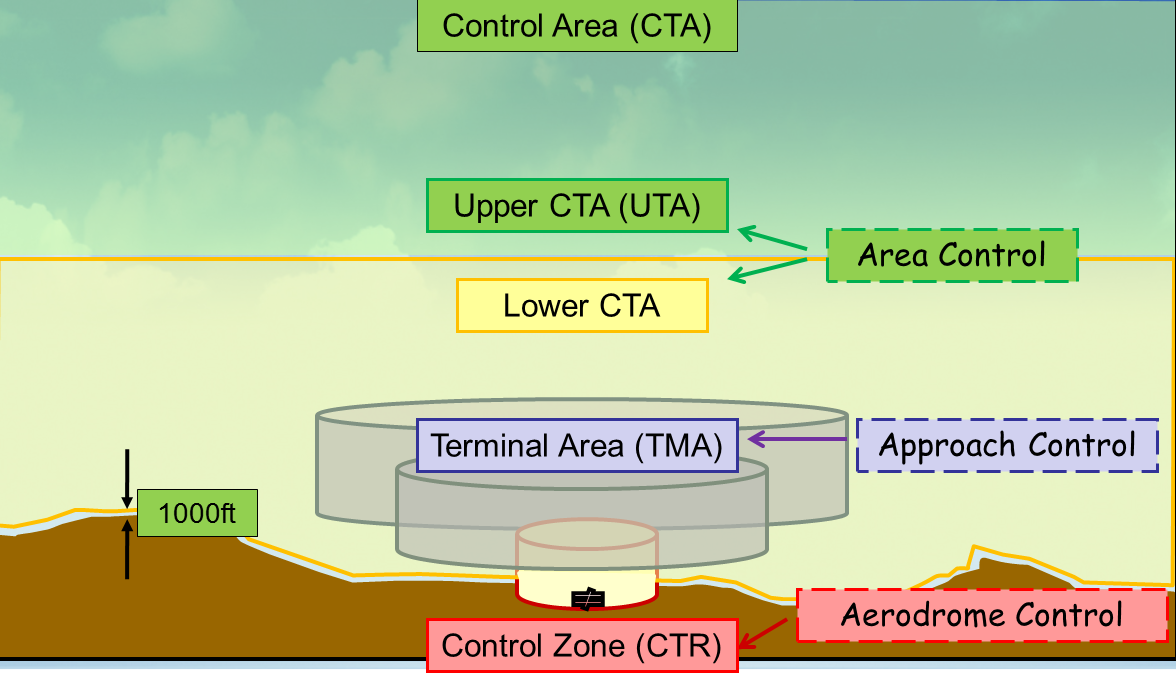
\includegraphics[width=0.8\textwidth]{figures/airspace2.png}
    \caption{Airspace - \textcolor{red}{z prezentace 2011 ATM Lesson Plans/ATM 1-2 General Air Traffic Control Service \cite[Chapter 2.10]{annex11} - překreslit!}}
    \label{fig:airspace2}
\end{figure}

\subsubsection{Area Control Service}
Area Control Service is an ATC service provided by area control centre (ACC) responsible for flights in Control Areas (CTA). Normally ACC is identified by the name of a nearby city, area or landmark. Smaller countries usually have one ACC, but many larger countries are controlled by several of them. ACCs usually control aircrafts in their en-route phase of flight. The ACC may be also responsible for flights to and from smaller aerodromes with no separate approach control service. \cite[Chapter 3.2]{annex11}

\subsubsection{Approach Control Service}
Approach Control Service (APP) is ATC service that is responsible for the part of CTA and CTR required by arriving or departing controlled flights (TMA). The primary functions of APP is sequencing arriving aircrafts and assisting departing aircrafts becoming established on course. The arrival and departure functions can be divided into several positions on busy aerodromes. APP is usually identified by the name of the aerodrome which it is serving, but sometimes it's not colocated with TWR and is at distant ACC location. When no separate ACC exists, approach control service is provided by ACC or TWR. \cite[Chapter 3.2]{annex11}

\subsubsection{Aerodrome Control Service}
Aerodrome control service is provided by a control tower (TWR) and is responsible for aircraft landing and taking off. It's also responsible for VFR flights in the CTR and for preventing collisions between aircrafts on the manoeuvring are of the aerodrome. \cite[Chapter 3.2]{annex11}

\textcolor{red}{z pohledu prostoru/z pohledu kontroly}

\textcolor{red}{v každou chvíli řídí letadlo jeden subjekt a místo a čas předání kontroly je jesně definované - kdy a jak?}

The controlled airspace can furthermore be classified as Class A-G. \cite[\textcolor{red}{kapitola}]{nolan} \textcolor{red}{popis jednotlivých classes podle nolana}

\textcolor{red}{Pro řízení v terminální oblasti nás zajímají všechny druhy řízení/prostoru, Agentfly má zatím jen ACC v CTA?}

\begin{figure}[h]
    \centering
    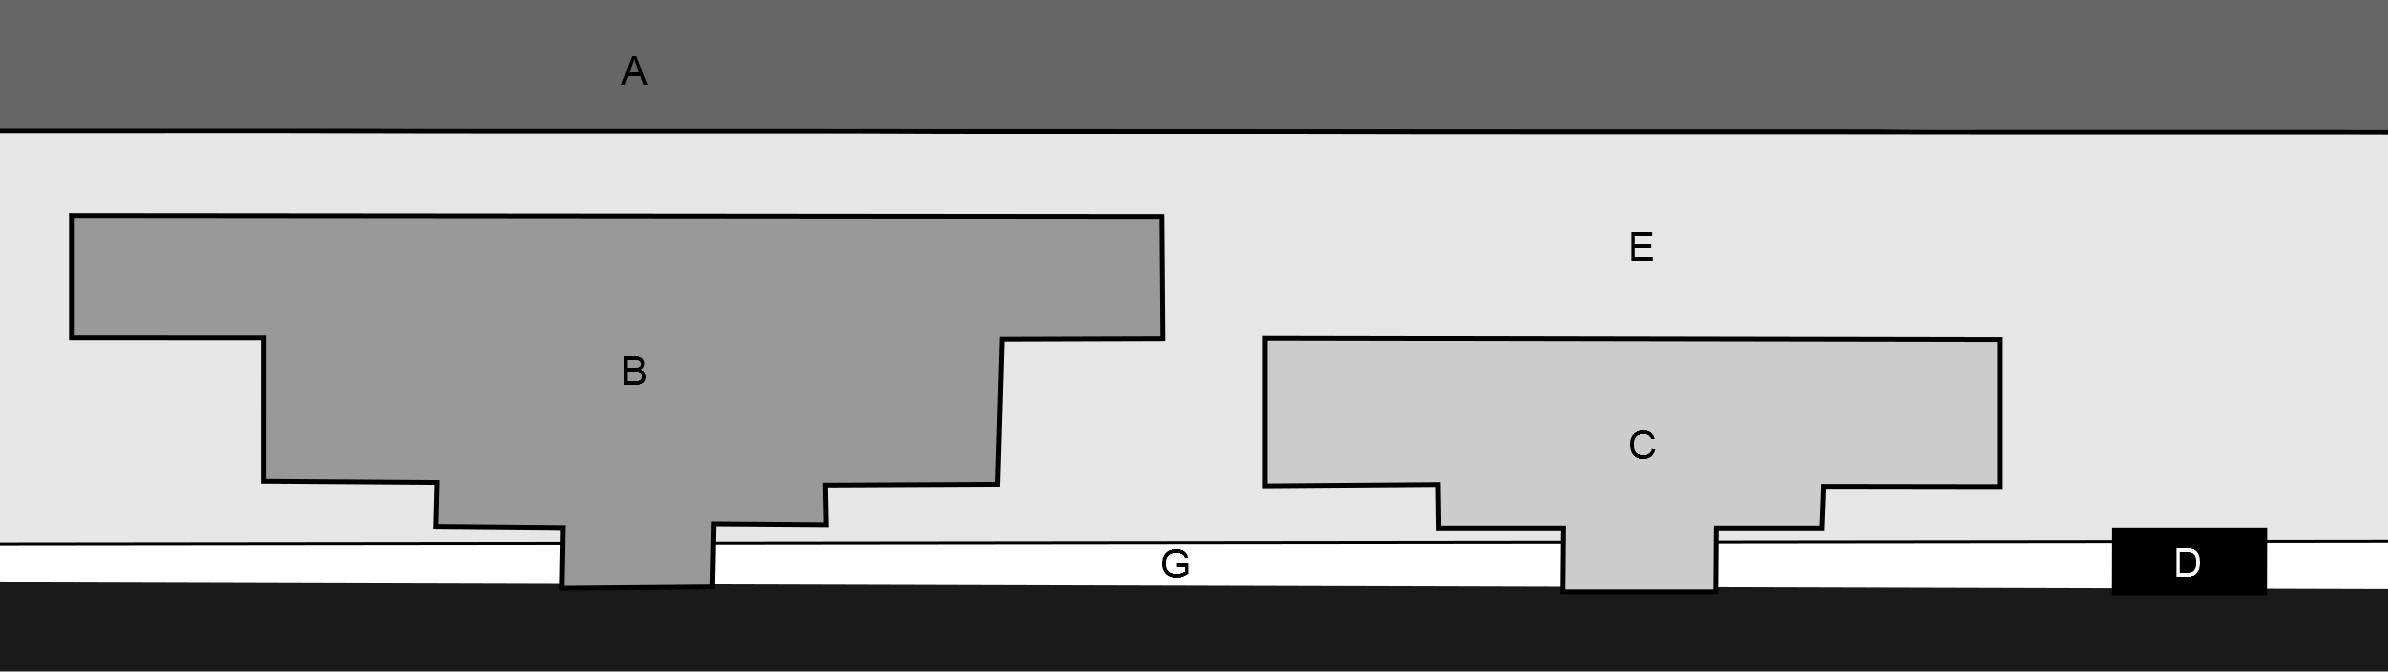
\includegraphics[width=0.8\textwidth]{figures/classes.png}
    \caption{Airspace Classification - \textcolor{red}{z prezentace 2011 ATM Lesson Plans/ATM 1-2 General Air Traffic Control Service \cite {nolan} - překreslit!}}
    \label{fig:classes}
\end{figure}

\textcolor{red}{SID a STAR routy?}

\subsubsection{Airspace Management}
ATM is generic term for any management activity for achieving the most eficient and flexible use of airspace avoiding permanent airspace segregation. \textcolor{red}{zdroj jen z prezentace}
The goals are to improve coordination between civil and military agencies, optimise route network and airspace structure and develop a free route airspace concept.

The concept of Flexible Use of Airspace (FUA) means that airspace should be treated as one continuous space that is being allocated according to user requirements. Any airspace segregation should only be temporary.

\subsubsection{Coordination within ATC}
unit $\leftrightarrow$ unit \\
ACC $\leftrightarrow$ APP \\
APP $\leftrightarrow$ TWR \\
sector $\leftrightarrow$ sector \\
sectors are within units

koordinaci mezi sektory popisuje \cite{doc4444} Doc 4444 Chapter 10
Detailed procedures are often subject to local regulations and rules.

Transferring unit/controller transfers the responsibility to control the aircraft to the accepting unit on point of transfer of control.

The transfer of control can be divided into three stages. First the flight is \bold{notified} to prepare for the transfer. Then the conditions of transfer of control are \bold{negotiated} with the transferring ATC unit and if necessary also with the accepting unit. After the parties \bold{agree}, the control is transferred to the accepting unit. his process can be achieved using automated means (AFTN, RDPS, FDPS, OLDI \textcolor{red}{?}) without using conventional telephone coordination. \textcolor{red}{(Jakože mezi sektory, s letadlem domluva asi pořád probíhá.)} \cite[Chapter 10.1.1]{doc4444}

This means that the flight is at any time under the control of only one ATC unit and can't be transferred from one unit to another without consent of the accepting unit. Also if communication with the aircraft is transwerred to the next unit, that unit cannot change the learance of the aircraft before the point of control transfer.

Doslovně z prezentace:
Control of an aircraft shall be transferred from ACC to APP, and vice versa, at a time or point agreed between the two units. This time or point is normally stated in a LOA.
Except when otherwise specified, APP may issue clearances to any aircraft released to it by ACC without reference to ACC. If an aircraft executes a missed approach, if necessary, ACC shall be informed immediately and subsequent action coordinated. 
After coordination with APP, ACC may release an arriving aircraft directly to TWR if the entire approach will be made under VMC.\cite[Chapter 10.1.3.1]{doc4444}

Doslovně z prezentace:
The take-off time is specified by the ACC when it needs to coordinate the departure with other ACC traffic or provide separation between other departing traffic on the same track. In other cases the APP determines the time of take-off so that the traffic in their AOR is separated. ACC and APP can also specify clearance expiry time if a delayed departure would cause separation problems. The time given by APP must not be later than ACC time. co je AOR?\cite[Chapter 10.1.3.2]{doc4444}

Doslovně z prezentace:
Exchange of movement and control data
APP shall keep ACC advised of data about controlled traffic such as:
RWY in use and type of instrument approach procedure;
lowest available level at the holding fix for use by ACC;
average time or distance intervals between successive arrivals as determined by APP;
revision of EATs as required (5 MIN or greater, or as agreed);
arrival times over holding fix when these vary by 3 MIN or greater from the times estimated by ACC;
flights cancelling IFR, if it will affect holding levels or EATs;
departure times, or if agreed, boundary or specified point times;
information relating to overdue or unreported aircraft; and
missed approach times which may affect ACC.
\cite[Chapter 10.1.3.3]{doc4444}

Doslovně z prezentace:
ACC shall keep APP advised of data about controlled traffic such as:
identification, type and point of departure of arrivals;
ETA and level of arrivals over holding fix or other specified point;
ATA and level of arrivals over holding fix if aircraft is released to APP after arriving over the holding fix;
requested type of instrument approach procedure if different to that specified by APP;
EAT issued;
when required, that an aircraft has been instructed to contact APP;
when required, that an aircraft has been released to APP, including if necessary, the time and conditions of release; and
anticipated delay to departures due to congestion.
ACC shall forward information on arrivals at least 15 MIN before ETA. \cite[Chapter 10.1.3.3]{doc4444}

Doslovně z prezentace:
Division of control
APP shall retain control of arrivals until the aircraft have been transferred to, and are in communication with TWR. Rules for transfer of control of arrivals shall be establish by LOAs or local instructions, considering airspace structure, terrain, MET conditions and ATS facilities available.
APP may authorize TWR to release a departure for take-off subject to the discretion of TWR with respect to arrivals.
TWR shall obtain approval from APP prior to authorizing SVFR flights, when so prescribed in LOAs or local instructions. \cite[Chapter 10.1.4.1]{doc4444}

Doslovně z prezentace:
Exchange of movement and control data
TWR shall keep APP advised of data about controlled traffic such as:
  arrival and departure times;
  when required, that the first aircraft in the approach sequence is in  	communication with and is sighted by TWR, and that reasonable 	assurance exists that a landing will be accomplished;
  information relating to overdue or unreported aircraft;
  information concerning missed approaches; and
  information concerning aircraft that are essential local traffic to aircraft 	under the control of APP.\cite[Chapter 10.1.4.2]{doc4444}


\textcolor{red}{konec 9-1 43}
%!TEX root = index.tex
\chapter{Data}

This chapter summarizes which data were used for implementation and testing of the module for air traffic control simulation in terminal area. The design and implementation of the module is general and can be used for simulation of any TMA sector but in order to test its functionality concrete sector description and air traffic scenario must be used. It was important to have all the data relevant to the test sector available because any of them missing would cause the whole scenario to be unusable.

\section{Hartsfield–Jackson Atlanta International Airport}

\begin{figure}[h]
    \centering
    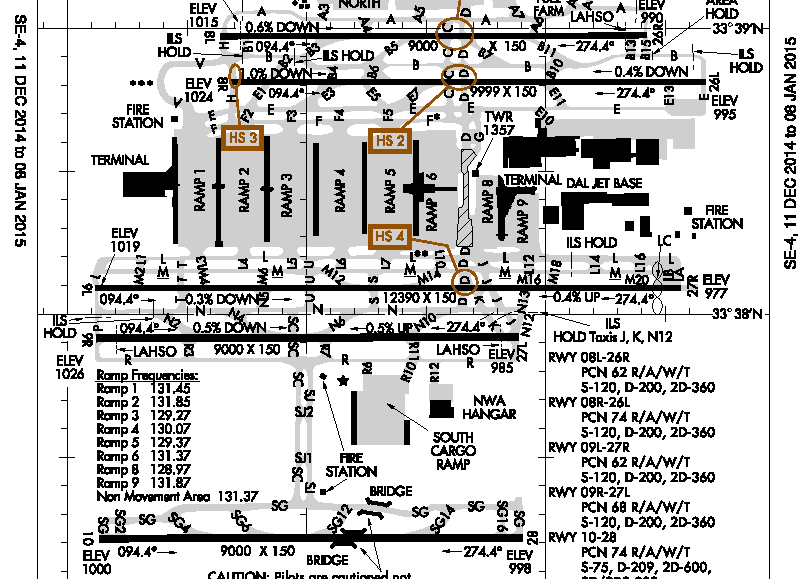
\includegraphics[width=0.8\textwidth]{figures/atlanta-diagram.pdf}
    \caption{Section of the airport diagram of the Hartsfield–Jackson Atlanta International Airport \cite{atlanta-diagram}}
    \label{fig:atlanta-diagram}
\end{figure}

Hartsfield–Jackson Atlanta International Airport (ICAO code KATL) has been the world's busiest airport by passenger traffic since 1998 with more than 94 million passengers in 2013. It has also the most landings and take-offs since 2005. The airport has 207 domestic and international gates which is the most at any airport. \cite{atlanta}

This airport was chosen because the amount of traffic would provide more interesting test-case in comparison to some other, less busy airport. Also all the other required data were available for Atlanta Airport.

The goal of this thesis is to simulate the approach phase of the flight, from the moment airplane leaves en-route sector to touchdown on the runway. The ground movement is not simulated and therefore the only information needed about the airport is the configuration of its runways.

The runway configuration is publicly available on the FAA website \cite{atlanta-diagram}. Airport runway configuration including positions and elevations of each runway was created in a form of XML file that can be used in AgentFly simulation.

The Atlanta Airport has five runways, the southernmost (\texttt{10/28}) is used for cargo aircraft and was therefore eliminated from the scenario. Out of the four remaining runways the inner two (\texttt{8R/26L} and \texttt{9L/27R}) are used exclusively for departures and only the outer two runways (\texttt{8L/26R} and \texttt{9R/27L}) are used for incoming flights. These two runways will be used in the test simulation scenarios. Figure \ref{fig:routes} shows all the Atlanta Airport runways (in yellow) as they are shown in AgentFly visualization.

\section{Atlanta TMA}

Together with the description of the Atlanta Airport itself, the definition of surrounding TMA sector was needed. This sector describes the area of authority of approach control service. The name of the TMA sector is \texttt{A80}. As the Atlanta Airport is one of the busiest airports, the associated TMA sector is defined as Class B airspace. The definition of the airspace is provided by Federal Aviation Administration \cite{atlanta-tma}.

\begin{figure}[H]
    \centering
    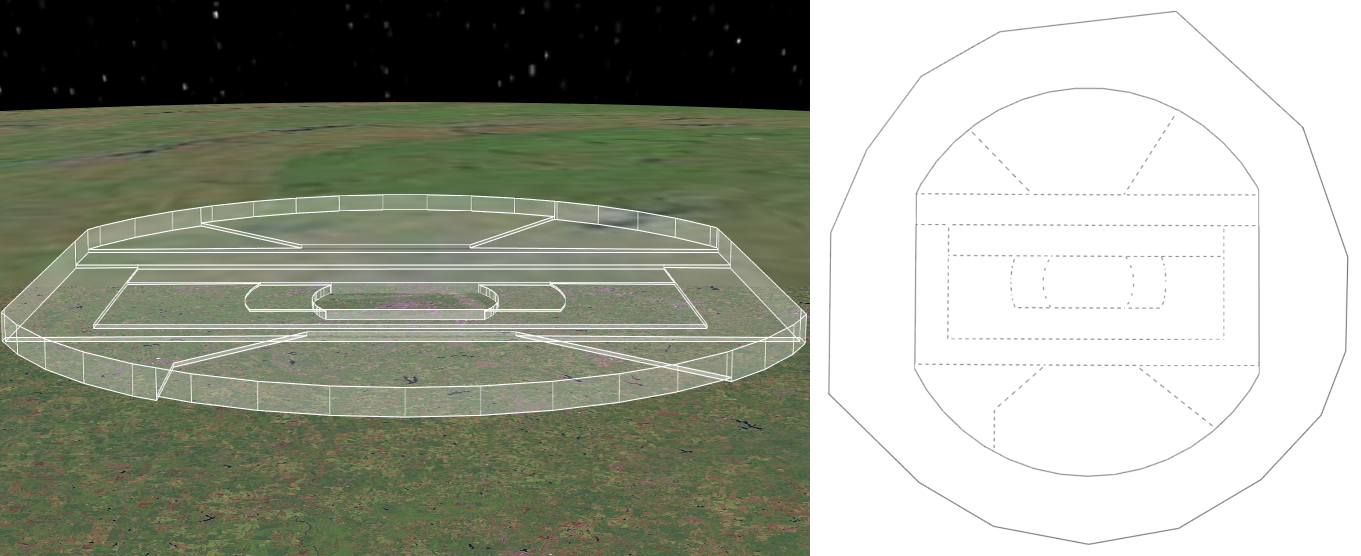
\includegraphics[width=\textwidth]{figures/tracon.png}
    \caption{Left: Atlanta Class B airspace in AgentFly 3D visualization, Right: The airspace as shown on radar screen in AgentFly with borders of neighboring en-route sectors}
    \label{fig:tracon}
\end{figure}

The definition of the airspace isn't available in a computerized form ready for machine processing and had to be converted to XML sector definition by hand from the available textual description \cite{atlanta-tma}. The resulting sector as seen in agentFly visualization is shown in Figure \ref{fig:tracon}. Problem with this TMA definition is that there is a gap between TMA border border and previously provided neighboring en-route sectors making it impossible to hand-off planes from one sector to the other. Upon consulting with FAA, for the purposes of testing the borders of surrounding en-route sectors were used for TMA definition  instead of the Class B airspace itself. This way the TMA sector touches the en-route sectors allowing airplane hand-offs. The comparison between Class B airspace and used sector definition is shown in Figure \ref{fig:tracon} right. The TMA sector and some neighboring en-route sectors is also shown in Figure \ref{fig:routes} left, note that the sectors do not overlap, the en-route sectors horizontally touch the TMA sector and partly extend above it.

\section{STARs}

STARs are routes that connect the en-route sectors and lead the airplanes to the runways. They define the path itself as well as safe intervals for altitude and speed for selected fixes on the route. The routes are designed in such way that if they cross horizontally, the separation is ensured vertically. This means that once a plane is flying on a STAR route there is no risk of collision with aircraft flying on other routes.

\begin{figure}[h]
    \centering
    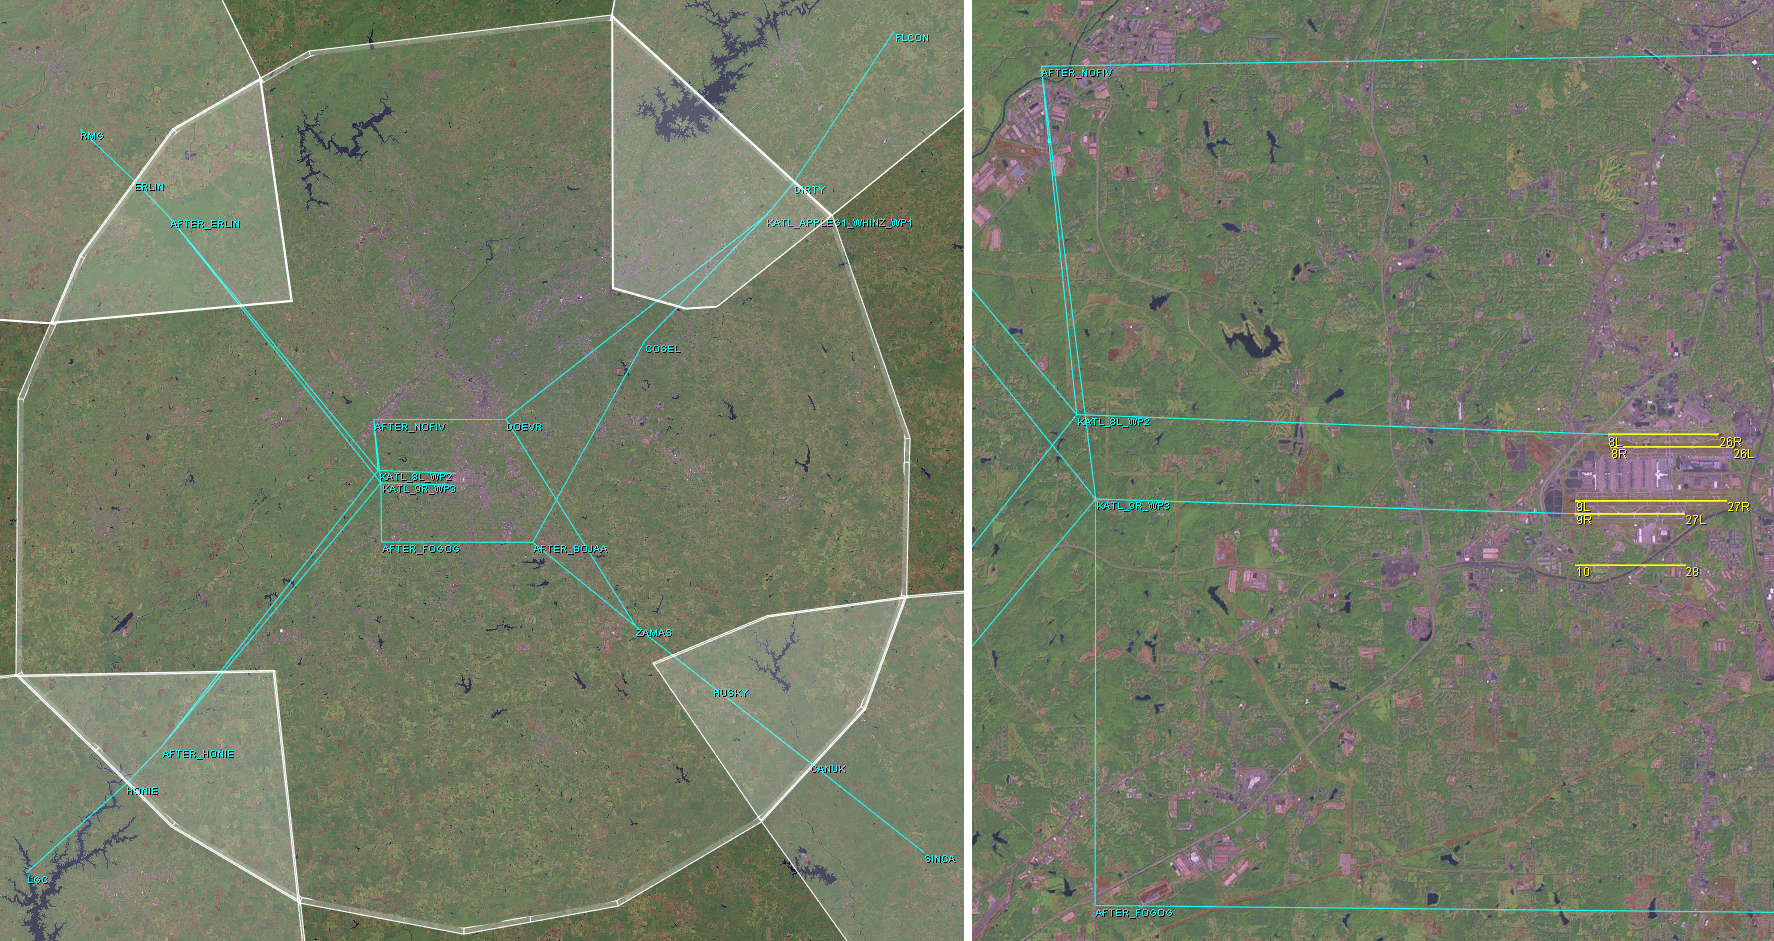
\includegraphics[width=\textwidth]{figures/routes.png}
    \caption{STARs near Atlanta Airport, Right: overall view, Left: detailed view of the configuration near runways}
    \label{fig:routes}
\end{figure}

The STAR definitions are made publicly available by the FAA in non-machine readable format but were also provided for the purpose of TMA simulation in AgentFly in computerized proprietary format. The provided STAR descriptions were used in this thesis even though they do not correspond entirely with the publicly provided data. SID routes were also provided but not used as simulation of takeoff was not part of the thesis.

Figure \ref{fig:routes} shows the loaded routes for eastern operation of Atlanta Airport in AgentFly visualization. Atlanta Airport can function in two configurations depending on the prevailing wind direction. The approaches and take-offs can be performed either in western or eastern direction. The route configuration is basically identical, only mirrored along the north-south axis. AgentFly doesn't simulate the wind at the moment and therefore static eastern direction was used for the testing purposes.

\section{Flights}

Recording of real-world 24 hour traffic in Atlanta Air Route Traffic Control Center (ZTL) on 20th June 2013 was provided by FAA for testing. The log files contain records of 7832 flights. Out of those VFR flights were filtered out because only IFR flights are simulated in AgentFly. Also aircraft of unusual type that can not be simulated using BADA simulation models were removed from the test data. Also flights flying through the \texttt{A80} sector or taking of at the Atlanta Airport were filtered from the logs leaving 1308 flights arriving to the airport.

\begin{figure}[h]
    \centering
    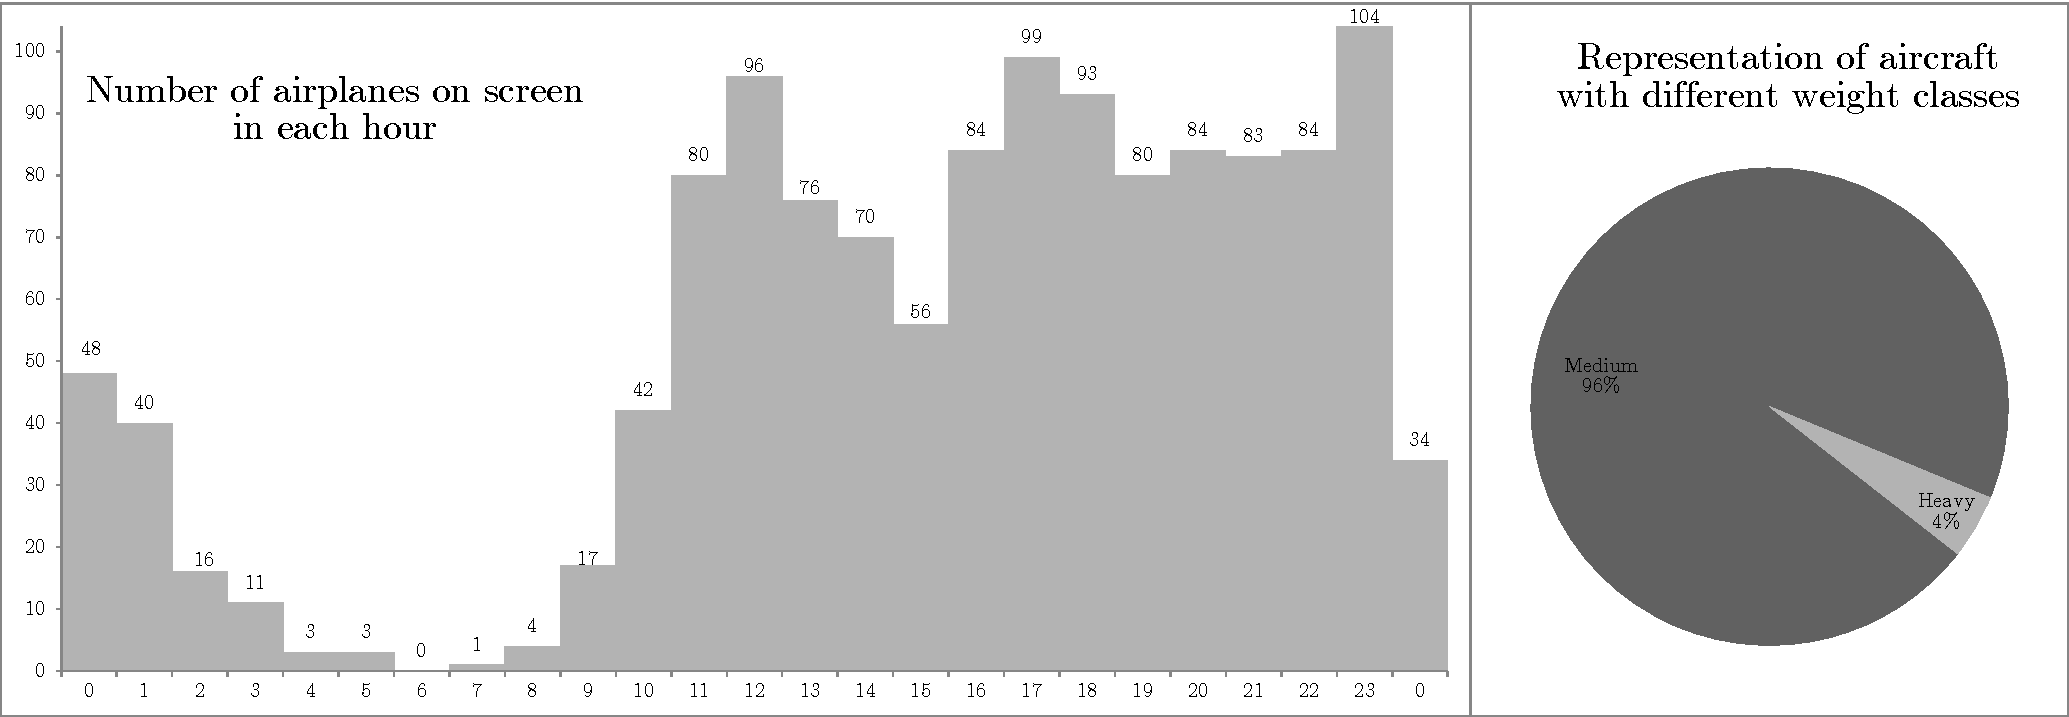
\includegraphics[width=\textwidth]{graphs/real-flights.pdf}
    \caption{Left: histogram of number of airplanes appearing on screen in each hour of the simulated 24 hours traffic, Right: graph of representation of aircraft with different weight classes in the test air traffic}
    \label{graph:flights}
\end{figure}

Figure \ref{graph:flights} shows the histogram of number of airplanes appearing on screen in each hour and graph of representation of aircraft with different weight classes in the air traffic. The histogram demonstrates the usual progress of the traffic during the day with decline in early morning and peaks around noon and in the evening. The pie chart shows that the traffic going to the Atlanta Airport is rather monotonous 96\% of medium weight aircraft, 4\% heavy aircraft and no light or super heavy planes. Therefore additional test scenario was created to test the scheduling algorithms in situations with more variable composition of arriving flights.
%!TEX root = index.tex
\chapter{AgentFly}

\section{Goal}

\section{Air Traffic Model}
\subsection{Pilot}
\subsection{Controller}
\subsubsection{ATA}
\subsubsection{RSide}
\subsection{Communication}
\subsection{Workload}

\section{Used Units}

\section{Competition}
\subsection{Boeing}
\subsection{...}
%!TEX root = index.tex

\chapter{Flights Scheduling}

\label{section:scheduling}

Main goal of this thesis is to design and implement algorithm for scheduling flights arriving to airport controlled by approach controller. This chapter defines the scheduling task and presents several algorithms that provide variety of approaches to solve the task. All of the algorithms were then implemented and experiments were conducted to find the most appropriate for real-world simulation.

\section{Term Definitions}

First, let's define some terms that will be used in this chapter:

\bitem
\item \textbf{ETA} – Estimated Time of Arrival to the runway if the airplane will fly directly without delay along given STAR.
\item \textbf{EETA} – Earliest ETA among all runways ariving flight may land on. If only one runway is available $\text{EETA}=\text{ETA}$. ETA is always bigger or equal to ETA.
\item \textbf{SETA} – Scheduled ETA is the time at which the airplane is scheduled to arrive to runway. SETA is always bigger or equal to ETA.
\item \textbf{Delay} – for single runway the delay of flight arrival is defined as $\text{SETA}-\text{ETA}$, for multiple runways the delay is defined as $\text{SETA}-\text{EETA}$.
\item \textbf{Slot} – time interval assigned to arriving flight on a runway. It is defined by SETA surrounded by buffer given by accuracy of the estimate.
\eitem

\section{Problem Definition}

The approach controller's main task is to schedule aircraft flying to an airport in controlled TMA sector, given following limitations:

\bitem
\item Individual flights arrive over time and the controller becomes aware of them at the time they appear on his/hers radar screen.
\item Each flight needs to be assigned one of available runways to land on and time interval in which the assigned runway is free.
\item The runway and slot assignment must be done at the time of their appearance on the radar screen, no flights are allowed to fly in the TMA sector not knowing which runway they will land on and when.
\item The slot must be scheduled to given estimated arrival time (ETA) or later.
\item Once the runway is assigned, it must not be changed.
\item Assigned slot may be rescheduled to a later time, it may not be rescheduled earlier.
\item The slots on single runway must be spaced at least by minimum wake separation interval length. The interval length depends on weight classes of both preceding and following airplane and on their order. This means that the separation interval of \textbf{Light} airplane behind \textbf{Heavy} airplane is different (longer) than interval of \textbf{Heavy} behind \textbf{Light}.
\eitem

\subsection{Existing Algorithms Solving Similar Problems}

The task the TMA sector controller deals with is a special case of online scheduling problem. There are several algorithms providing solutions for variety of online scheduling problems \cite{scheduling}, but none were found, that would be applicable for this scheduling task. Some of the algorithms allow for jobs (corresponding to arrival slots) to wait before being assigned to one of available machines (corresponding to runways) which is not possible here. Other make the allocation of jobs to machines irreversible, in flight scheduling problem the machine (runway) selection is irreversible, but the job order on the runway is variable (with the restriction that jobs mustn't be rescheduled earlier). Some algorithms allow job preemption which is not allowed in flight scheduling. There are algorithms that allow temporal constraints between jobs, but the constraints are static, here the temporal constraints are dynamic, they only apply for jobs scheduled directly behind each other on single machine and depend on the job's order. Additionally the algorithms search for optimal solution according to single criterion, whereas in flight scheduling we look on several performance criteria and don't search for optimal result but try to find good solution by as many criteria as possible.

\subsection{Evaluation Criteria}

The criteria the TMA sector controller takes into account while scheduling approaching flights are following:

\bitem
\item \textbf{Makespan} – the length of scheduled runway plan, which is equal to the difference between SETA of last and first task on the runway. For multiple runways the makespan is defined as difference between SETA of last and first task among all runways. Makespan expresses the quality of the schedule in terms of system efficiency and airport throughput and safety, as plan with shorter makespan leaves more leeway for future arriving airplanes in case of unexpected increase in the incoming traffic.
\item \textbf{Total delay} – sum of all delays of scheduled arrivals. It expresses the schedule quality in terms of social welfare as lower total delay means lower fuel consumption and thus lower costs for airlines and lower emissions.
\item \textbf{Maximal delay} – maximal delay among all scheduled arrivals. It expresses the plan quality in terms of competitive welfare and safety as too long delay may cause the airplane to deplete it's fuel supply before landing and therefore lead to an accident. Also no airline want their flight to wait while other flights are landing and therefore more uniform delay distribution among all flights is desirable.
\item \textbf{Number of replanned slots} – total number of replanned slots during the scheduling (one slot may be replanned multiple times after additional slot allocations). It expresses the plan quality in terms of controller workload and safety as high number of changes in planned slots require the controller to update the instructions given to pilots and thus increasing his/hers workload.
\eitem

Because no existing algorithm providing desired properties was found, algorithms were designed specifically for the flight scheduling problem. The problem was divided to two parts. First, new slot is allocated on all available runways and then the resulting plans are compared and one runway is selected. This way the algorithm produces both slot and runway allocation. Algorithms for both parts of the problem are proposed in following sections but first visual representation of the runway plan is described so it can be used later to illustrate the outputs of individual algorithms.

\section{Runway Plan Visualization}

\label{section:runway-visualization}

Runway Plan Visualization module was designed to provide representation of the runway plan that is quick and easy to comprehend. The slots planned for approach are displayed horizontally with a timeline at the bottom with highlighted one and five minute marks.

Above the timeline there are rows representing individual runway plans. Headline of each runway plan is shown on the left side with the number of the runway on the top and names of every weight class in corresponding color shown below. Plans of different runways planned by the same algorithm are divided by gray dashed border. Plans of different runways planned by different algorithms are divided by solid black border.

Each slot in the plan is represented by a vertical green bar with a dark green line in it. The dark green line shows the exact time of SETA and the green bar surrounding it shows the interval of possible arrival as defined by the precision of arrival estimation. Flight ID is shown on the top, the color of the text indicates the weight class of the aircraft. Below the flight ID, gray wake turbulence intervals are shown for every weight class in the same order as in the plan headline. If the wake turbulence interval is active (there is an following airplane scheduled after the current slot), the corresponding interval is colored in the color of following airplane's weight class.

If there is a collision between the slots, active wake turbulence interval of the preceding slot and the slot itself of the following flight are shown in red color. If a slot is delayed, vertical orange line marks the time of original ETA and is connected to the delayed ETA with horizontal orange line. In multi-runway scenarios, earliest ETA among all runways (EETA) is marked by dotted orange line and is again connected with the delayed ETA with horizontal dotted line. This way the controller can distinguish which part of the delay is caused by the order of slot on the runway and which part of the delay is the runway selection responsible for.

Examples of algorithm outputs shown in this chapter are results generated by individual algorithms for scenario defined in Table \ref{tab:config-simple}. The scenario was chosen specifically to illustrate different results produced by the algorithms.

\begin{table}[h]
  \centering
\begin{tabular}{ | l | c | r | r | }
\hline
Flight id   & Weight class & Appearance on screen & Estimated arrival time \\
\hline
01          & MEDIUM       & 14:48                & 48:09 \\
02          & MEDIUM       & 17:36                & 44:23 \\
03          & JUMBO        & 19:00                & 46:11 \\
04          & JUMBO        & 19:24                & 44:11 \\
05          & MEDIUM       & 21:36                & 48:23 \\
\hline
\end{tabular}
  \caption{Configuration of the scenario illustrating different outputs generated by individual algorithms}
  \label{tab:config-simple}
\end{table}

\section{Slot Allocation on Single Runway}

\label{section:slot-selection}

This section presents several algorithms designed to allocate arrival slot on single runway. The input of the algorithm is ETA, airpane's weight class and slot size, output is the runway plan with new allocated slot.

\subsection{Algorithm 0 – Force Slot on ETA}

\begin{figure}[h]
    \centering
    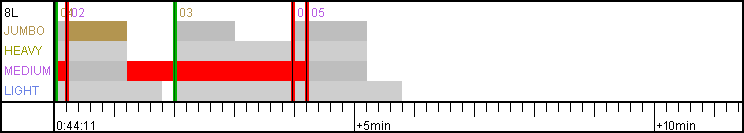
\includegraphics[width=\textwidth]{figures/rwy-in-place.png}
    \caption{Example of runway plan with colliding slots}
    \label{fig:rwy-in-place}
\end{figure}

An example of a plan generated by Algorithm 0 is shown in Figure \ref{fig:rwy-in-place}. This algorithm is the simplest of all implemented, it doesn't perform any deliberation on where to put the slot in the plan and simply places it in the time the aircraft is expected to arrive, ignoring possible collisions with other aircraft. This algorithm is not intended for actual use and serves only for comparison to other algorithms and to allow analysis of the traffic flow: it shows how many collisions there are or if the airplanes arrive to the runway periodically or in groups.

\subsection{Algorithm 1 – Keep Order of Appearance on Radar}

\begin{figure}[h]
    \centering
    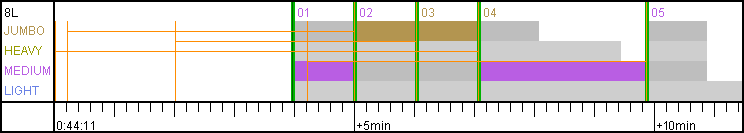
\includegraphics[width=\textwidth]{figures/rwy-end.png}
    \caption{Example of runway with slots in the order of airplane's first appearance}
    \label{fig:rwy-end}
\end{figure}

Algorithm is a simple first-come, first-served algorithm that produces valid plans with no collisions between slots. When new airplane appears on radar screen it's slot is created after all previously planned slots and not sooner than at the airplane's ETA.

Figure \ref{fig:rwy-end} shows an example of a plan generated by this algorithm. It is clearly visible that unnecessary delays can occur when the interval between the time when the airplane shows on the radar and its ETA differ from airplane to airplane. This can happen when the arrival routes have different lengths. Approach route for airplane heading directly to runway will be much shorter than for airplane arriving from opposite direction, because such airplane must first fly around the airport before landing. See Figure \ref{fig:routes} for example, the routes from south-west are significantly shorter than routes from south-east. In the example plan shown in Figure \ref{fig:rwy-end} flight \texttt{04} will arrive more than 7 minutes late because it appeared on the radar screen later than flights \texttt{01}, \texttt{02} and \texttt{03} even though its ETA is smallest.

\subsection{Algorithm 2 – Find First Empty Space in Which The Slot Fits}

\begin{figure}[h]
    \centering
    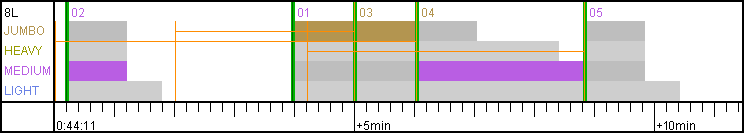
\includegraphics[width=\textwidth]{figures/rwy-fill-voids.png}
    \caption{Example of runway plan with slots fixed in place}
    \label{fig:rwy-fill-voids}
\end{figure}

Algorithm 2 creates the slot for arriving airplane in the first empty space following airplanes ETA in which the slot fits. The wake turbulence separation minima is taken into account for both preceding and following slot so no collisions between slots occur. The advantage of this this algorithm is its simplicity and the fact that the planned slots are fixed. This means that if the controller assigns a slot to airplane and clears it for approach he/she doesn't have to alter the airplane's clearance and can focus on other arriving aircraft.

An example of a plan generated by Algorithm 3 is shown in Figure \ref{fig:rwy-fill-voids}. In comparison to plan generated by previous algorithm (\ref{fig:rwy-end}) it is apparent that flight \texttt{02} can land sooner than \texttt{01} even though it entered the controlled area later. However \texttt{03} and \texttt{04} won't fit the void between \texttt{02} and \texttt{01}, and must be scheduled after. \texttt{05} would fit but arrives to the runway too late.

\subsection{Algorithms 3a, 3b – Keep Order of ETA (With Local Optimization)}

\begin{figure}[h]
    \centering
    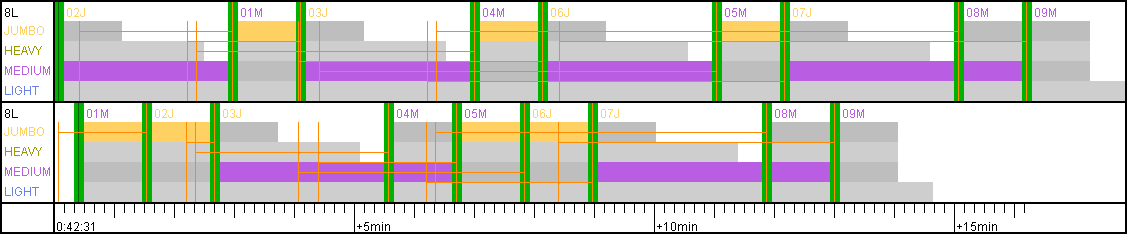
\includegraphics[width=\textwidth]{figures/rwy-eta-order.png}
    \caption{Example of runway plan that preserves the order of ETA}
    \label{fig:rwy-eta-order}
\end{figure}

Third algorithm was implemented in two variants, the first one ({\em 3a}) schedules the slots in a way that strictly preserves the order of estimated time of arrival. If the slot doesn't fit, any already planned slots following this one are delayed. If there is a continuous stream of airplanes scheduled for approach one after other and new, early arriving airplane appears on the radar screen the controller using this algorithm will squeeze the airplane in and postpone all airplanes following in the stream. This prevents a situation where the new airplane would wait for all the airplanes in the stream to land first. On the other hand the controller may need to postpone a significant number of previously planned aircraft which would take a considerable amount of time.

The second variant ({\em 3b}) is not strict with the order according to ETA. It finds the place where the new slot would fit by the ETA, but inserts it only if the delay of the following slot after the new slot is inserted is smaller than the delay of the new slot would be if it was placed after the following slot. Otherwise it tries to insert the new slot after the slot following it and so forth until the condition is met. This serves as a local optimization of the maximal delay and helps the algorithm to cope with flights with alternating weight classes.

The example plans generated by this algorithm are shown in Figure \ref{fig:rwy-eta-order}, first row contains result of variant ({\em 3a}), second row contains variant ({\em 3b}). The difference between the algorithms is visible on the order of \texttt{02} and \texttt{04}. \texttt{02} is planned first (from these two) directly on its ETA. When the \texttt{04} was inserted into the plan, variant {\em 3a} placed it before \texttt{02} because its ETA is smaller. Variant {\em 3b} with the local optimization compared the delay of \texttt{02} behind \texttt{04} with delay of \texttt{04} behind \texttt{02} and find out that the second one is smaller and therefore pushed \texttt{04} behind \texttt{02}. Before placing \texttt{04} it compared it with \texttt{03} and when delay of \texttt{03} behind \texttt{04} was smaller than the other way around it placed the slot \texttt{04} between \texttt{02} and \texttt{03}.

\subsection{Algorithms 4a, 4b, 4c – Branch And Bound}

\begin{figure}[h]
    \centering
    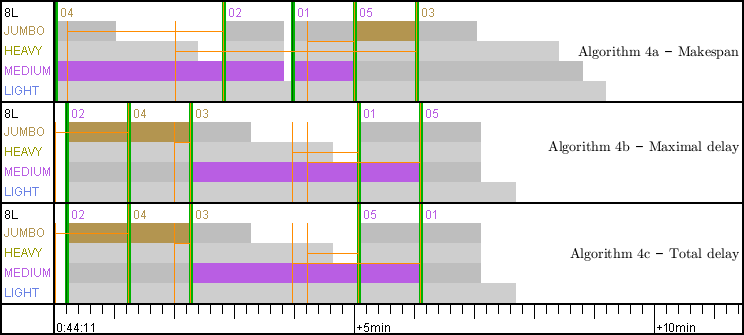
\includegraphics[width=\textwidth]{figures/rwy-bab.png}
    \caption{Comparison between the three variants of Algorithm 4}
    \label{fig:rwy-bab}
\end{figure}

Algorithm 4 is an algorithm commonly used in combinatorial optimization and is called Branch and bound. \cite{bab} The algorithm is used here in three different variants, each optimizing different criterion. Variant {\em 4a} minimizes makespan.  Variant {\em 4b} minimizes maximal delay. Variant {\em 4c} minimizes the sum of delays of all planned slots.

Figure \ref{fig:rwy-bab} shows a comparison between the three variants of Algorithm 4. It shows that the variant {\em 4a} indeed produces plan with smallest makespan but with big delays for some slots. {\em 4b} and {\em 4c} produce plans with same total delay but {\em 4b} has smaller maximal delay.

\begin{figure}[h]
    \centering
    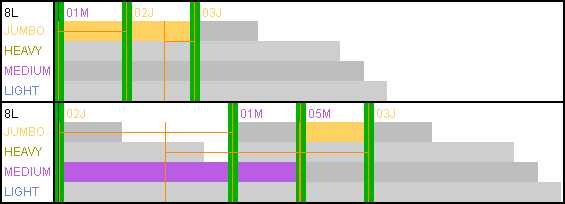
\includegraphics[width=0.7\textwidth]{figures/rwy-proof.png}
    \caption{Example of adding later slot causing changes in plan before its ETA, first row shows plan before addition of slot \texttt{D}, second row shows plan after addition}
    \label{fig:rwy-proof}
\end{figure}

There are two disadvantages of branch and bound algorithm that limit its use in real world applications.

The first one is that it doesn't keep the relative order of previously planned slots. This is caused by the fact that the algorithm is an offline algorithm and recomputes the whole plan from scratch every time new slot needs to be added. This is illustrated in Figure \ref{fig:rwy-proof} where addition of slot for flight \texttt{D} caused the order of slots for \texttt{A}, \texttt{B} and \texttt{C} to change. Changing the order of flights scheduled on a route to one runway would result in need of special behavior that would allow the airplane to leave the route, wait in a separate area until the following aircraft flies past on the route and then return back to the route. And because the complete replanning takes place every time new airplane appears on a screen it could happen that two flights would switch their place in the sequence back and fort multiple times before reaching runway.

Additionally the planned delay may decrease for any given airplane in time (see \texttt{B} in Figure~\ref{fig:rwy-proof}). But if the airplane already performed certain manoeuvre to slow it down to accommodate the delay prescribed by the previous plan, it may be impossible to speed up to reach the runway in time planned by the updated plan, even if it would be able to do so before the hold-up.

\begin{table}[h]
  \centering
\begin{tabular}{ | l || r | r | r | r | r | r | }
\hline
			& 10 slots	& 11 slots	& 12 slots	& 13 slots	& 14 slots	\\
\hline
4a – Makespan	& $< 1s$	& $3s$		& $37s$		& –			& –			\\
4b – Maximal delay	& $< 1s$	& $< 1s$	& $< 1s$	& $7s$		& $33s$		\\
4c – Total delay	& $< 1s$	& $4s$		& $45s$		& –			& –			\\
\hline
\end{tabular}
  \caption{Run times of the three variants of Branch and bound algorithm}
  \label{tab:alg5-runtime}
\end{table}

The second disadvantage of this algorithm is also linked to the need to recompute the whole plan with each slot addition and it is the computational complexity of the Branch and bound algorithm.

The algorithm enumerates possible solutions in a systematic way that ensures the optimum will be found eventually. To prevent searching through the whole state space, upper and lower bounds are used to prune the unpromising branches from the search tree. The minimal solution found so far can act as an upper bound pruning all branches with partial plans whose criterion value is already bigger or equal to the optimum. This is especially beneficial for the second variant minimizing maximal delay among all slots, because the pruning takes place early on in the search tree, eliminating many non-optimal solutions.

For optimizing makespan any empty voids in the plans can be used as a bound for the solution. This can be done if the slots are ordered according to their ETA. In such case if the ETA of the next added slot is later than the end of the previous slot and forms an empty void before it, the optimal solution lies in a tree rooted by the added slot. This is because rearranging the order of previous slots wouldn't allow the next slot to start sooner than it starts in the current partial solution. This bound cannot be used in variants 2 and 3, because rearranging previously planned slots can still improve maximal and total delay.

The sum of tasks that remain to be planned added to the length to the current partial plan can serve as an upper bound to the solution. If this value exceeds the value of the minimal solution found so far it is obvious that planning the remaining tasks cannot result into better result and current sub-tree can be pruned. This bound cannot be effectively used in this planning problem, because the size of the slots isn't constant and therefore the size of the sum depends on the order in which the slots are added to the plan. And finding the order of the slots that produces the smallest sum equals to the planning problem itself.

The previously mentioned restrictions limit the benefits of pruning and the algorithm must therefore search through a significant part of the state space which makes it slow. The Table \ref{tab:alg5-runtime} shows the runtime for rather small instances of the planning problem. The algorithm would not be useful for faster than real time simulation as is, but may serve as reference algorithm for small instances or in combination with online planning algorithm (for example for local optimization run on several neighboring slots around newly added one). 

\section{Runway Selection}

\label{section:runway-selection}

When the configuration of STARs and the airport allows the airplanes to land on one of several runways, the air traffic controller must not only decide on the order in which the airplanes land on the runway but also on which airplane lands on which runway.

The procedure for runway selection goes as follows: For every runway the arriving airplane can land on, new plan is created incorporating the slot for the incoming airplane. The plans are created using the single-runway algorithms introduced in previous section. Then all the created plans are compared using one of the criteria presented below and the optimal plan is used for the corresponding runway.

\bitem
\item First criterion used to compare runway plans is the number of slots on each runway. The plan with \textbf{less slots} is selected. This will keep the number of slots on runways balanced leading to even distribution of flights between runways.

\item Second criterion guides the airplane to the runway with the \textbf{smallest makespan} after the slot addition. This is another way of balancing the flights between the runways, this time taking into account the arrival times and not only number of slots.

\item Third criterion selects the runway with smallest \textbf{maximal delay} of slots planned on the runway. Note, that for multiple runway scheduling delay is defined as difference between SETA and EETA.

\item Fourth criterion for runway selection is \textbf{total delay} of all slots on the runway, again delay is defined as SETA minus EETA in this case. 

\item Last criterion used to compare runway plans is \textbf{SETA of the new slot}. The air traffic controller wants the airplanes to land as soon as possible and this criterion is focused on that. It compares the scheduled arrival times of the newly added slot and directs the airplane to the runway with lowest time. This way the airplane may fly to a runway which is further away if the runway is less utilized and allows for earlier landing than a runway that has the shortest route.
\eitem

All algorithms were implemented in AgentFly system and then different combinations of slot allocation and runway selection algorithms were evaluated to determine which combination is best suitable for simulating real-world scenarios.
%!TEX root = index.tex
\chapter{Implementation}

\red{TODO}

\section{Scheduling}

\red{TODO}

\begin{algorithm}[H]
\begin{algorithmic}
\renewcommand{\algorithmicrequire}{\textbf{Input:}}
\renewcommand{\algorithmicensure}{\textbf{Output:}}

\Function{newAirplaneOnScreen}{plane}
	\If{plane isn't heading to the airport}
		\State \Return
	\EndIf
	\State \red{todo}
\EndFunction
\end{algorithmic}
\caption{Processing new airplane on screen}
\label{alg1}
\end{algorithm}

\section{STAR Application}
\subsection{Flight Plan update}
\subsection{Clearances}
\subsection{Speed}

\section{TMA to Enroute Communication}

\section{Flow Control}
\subsection{Vectoring}
\subsection{Holding Pattern}
\subsection{Miles In Trails}

\section{Runway Plan Visualization}

% přivádím až k letišti ale poslední úsek jen tak nahrubo, pak ho odřídí tower

% přesnější popis zadání - so teda chci dosáhnout

% Class B airspace Around atlanta
% vytvořeno z dostupných informací - popsat tam slovně ten tvar?
% obrázky
% vnější obvod aby seděl na dané sektory
% informace o update tvaru

% první update:
% http://www.dot.ga.gov/localgovernment/intermodalprograms/aviation/documents/classbpresentationshowformat.pdf
% http://proofofright.files.wordpress.com/2011/07/atl-class-b1.jpg

% druhý update:
% http://web.co.dekalb.ga.us/pdkairport/pdf/AirspaceArticle.pdf
% asi aktuální verze:
% https://www.federalregister.gov/articles/2012/02/03/2012-2072/proposed-modification-of-the-atlanta-class-b-airspace-area-ga !!!!!!!!!!!!!!!!!!!!!

% nejdřív zkoušení funkčnosti na doplňku, pak na class 2 airspace, protože pod ním se nacházejí další letiště (12, v okolí dalších 11) -> menší prostor -> komplikovanější



% definice samotného letiště,
% v tuhle chvíli stačí runwaye
% podle
% http://airnav.com/airport/KATL a http://155.178.201.160/d-tpp/1410/00026AD.PDF

% dát tam samotný popis runwayí, obrázek konfigurace, co jsme vyignorovali (povrch, navádění atd.), screenshot z visia 





% vytvoření nové konfigurace, vyfiltrování letů, které letí z/do/přes atlantu

% popis výběru a napasování route na FP
% jak se řeší napasování routy když jde souběžně ale po jiných fixech, viz ASQ5502_798


% eventy, skenování, radio, přeplánování, update fpi a horizontálního plánu

% porovnání s online schedullingem, kde můžou tasky čekat dokud se procesor neuvolní, ale tady se musí vykonávat od začátku, protože jinak letadlo spadne

% generování volných slotů: co nejdřívější, bere se ohled na nepřesnost odhadu ETA a marginy na obou stranách, z nichž má přednost ten delší
%!TEX root = index.tex
\chapter{Testing}

\red{TODO: intro}

\section{Comparison of scheduling algorithms on single runway}

This first test compares the performance of implemented scheduling algorithms. The scenario contains twelve flights with alternating weight class landing on one runway arriving in close succession. This scenario should be particularly demanding to be scheduled optimally because the alternation in weight classes make it sensitive to the order in which the slots are scheduled.

\begin{table}[h]
  \centering
\begin{tabular}{ | l | c | r | r | }
\hline
Flight id	& Weight class	& Appearance on screen & Estimated arrival time	\\
\hline
01M	& MEDIUM	& 17:36	& 42:30	\\
02J	& JUMBO		& 19:24	& 42:29	\\
03J	& JUMBO		& 19:00	& 44:15	\\
04M	& MEDIUM	& 22:00	& 44:49	\\
05M	& MEDIUM	& 21:36	& 46:30	\\
06J	& JUMBO		& 23:24	& 46:29	\\
07J	& JUMBO		& 23:00	& 48:15	\\
08M	& MEDIUM	& 26:00	& 48:49	\\
09M	& MEDIUM	& 25:36	& 50:30	\\
10J	& JUMBO		& 27:24	& 50:29	\\
11J	& JUMBO		& 27:00	& 52:15	\\
12M	& MEDIUM	& 30:00	& 52:49	\\
\hline
\end{tabular}
  \caption{The configuration of the first test scenario}
  \label{tab:config1}
\end{table}

Table \ref{tab:config1} shows the configuration of the test scenario. For the \texttt{JUMBO} category the Airbus A380-800 was used and the \texttt{MEDIUM} category was represented by Boeing 737. Airplanes headed to the airport from two separate streams to prevent possible violation of separation in en-route sectors the planes fly from.

\begin{figure}[h]
    \centering
    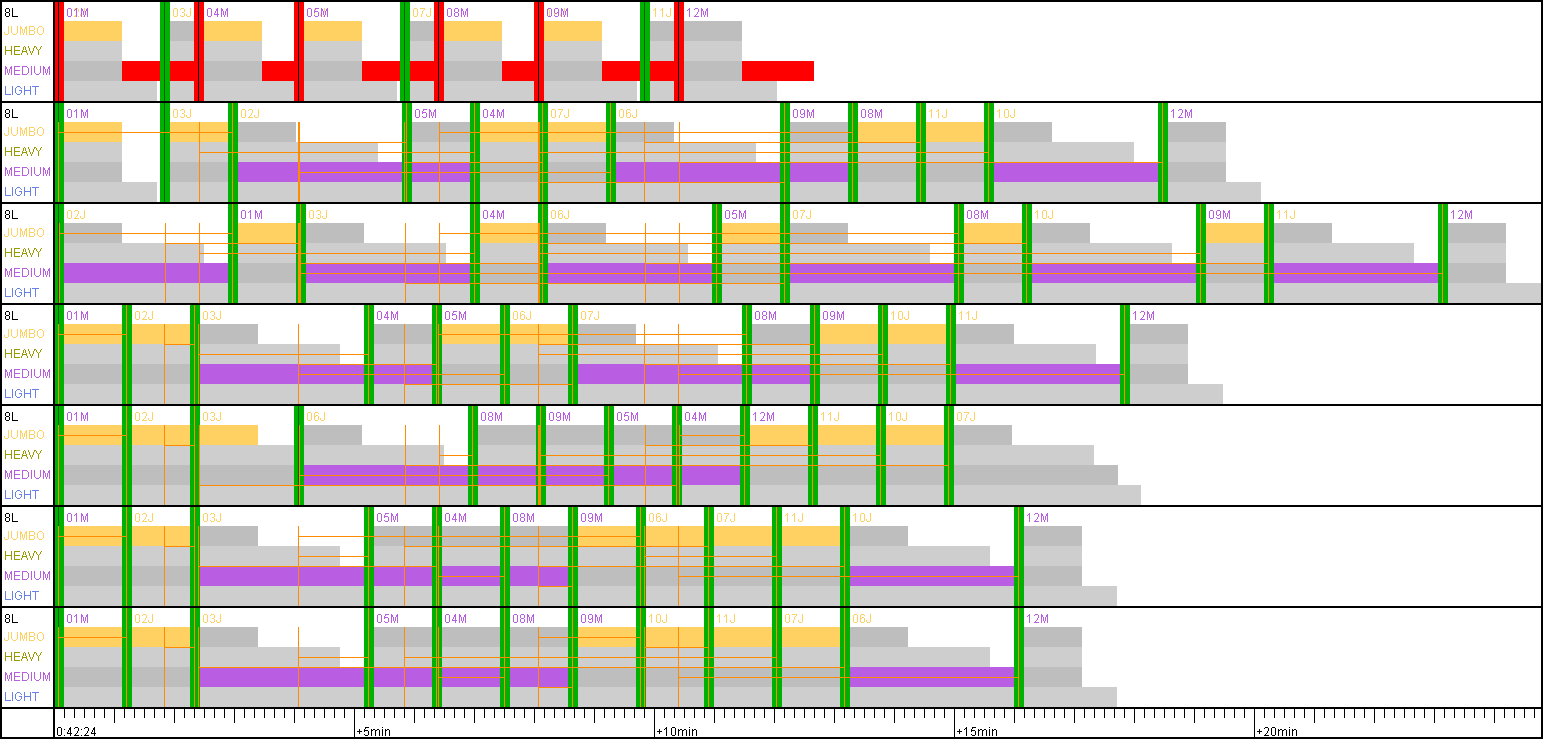
\includegraphics[width=\textwidth]{figures/1rwy-alternating.png}
    \caption{Result of planning with different algorithms on single runway}
    \label{fig:1rwy-alternating}
\end{figure}

The resulting plans are shown in Figure \ref{fig:1rwy-alternating}. The first row shows the result of {\em Algorithm~1} which places the slots in the exact time the arrival was estimated. It demonstrates how many collision would occur if no planning was present and serves as the lower bound on the total plan time.

The plans generated by {\em Algorithm~2} and {\em Algorithm~3} are identical in this case and are depicted in the second row. The slots are ordered in the same succession the corresponding aircraft appeared on the controller's screen. The reason the plans are identical is that the stream of arriving planes is very dense and there are no voids present between the aircraft the {\em Algorithm~3} would utilize to produce better schedule than {\em Algorithm~2}.

Third and fourth rows show the results of both versions of {\em Algorithm~4}. The third row contains the plan generated by the simple version of the algorithm, that keeps the order of aircraft's expected time of arrival. In this instance the algorithm produced the poorest result with the longest overall time as well as longest maximal and total delays. This is due to the specific configuration of the test scenario that alternates between weight classes. The second version doesn't rigorously keep the order of estimated arrival but tries to locally minimize the delays and therefore produces much better result.

The last three rows contain plans generated by the three versions of {\em Algorithm~5}. Each one shows optimal plan according to selected criterion. The one in the fifth row has the shortest total makespan. The plan in sixth row has the shortest maximal delay of a slot in the plan. And the last plan has minimal sum of delay of all slots. Note, that the last two plans are very similar and even have the same total length but the order of the slots determines whether the solution minimizes one or the other criterion.

\subsection{Makespan}

\begin{figure}[h]
    \centering
    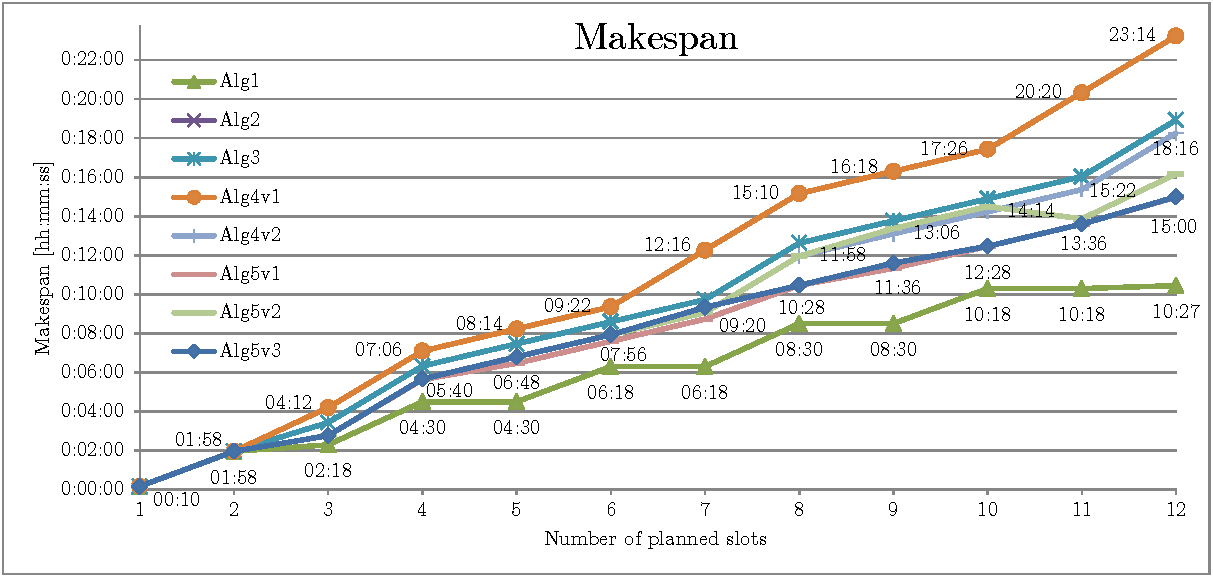
\includegraphics[width=\textwidth]{graphs/1rwy-alternating-makespan.pdf}
    \caption{Graph of makespan for plans created with different algorithms on single runway}
    \label{graph:1rwy-alternating-makespan}
\end{figure}

The obvious criterion by which the quality of a plan can be determined is the total duration of the schedule, also called makespan. The shorter the plan is, the better, because all the planes will in total land in the shortest possible time. In reality this criterion is problematic, because the flow of airplanes to the airport is infinite, only the density changes in time. But even so, this criterion can give a notion of the quality of immediate plan.

Makespan times in the progress of planning are shown in Graph \ref{graph:1rwy-alternating-makespan}. The result given by {\em Algorithm~1} is a lower bound that is given by the configuration of the testing scenario, no plans can be shorter than this value. The longest plans are generated by {\em Algorithm~4v1}. Plan with minimal makespan is generated by {\em Algorithm~5v1}, with {\em Algorithm~5v3} having very similar results (the values for 12 planned slots differ by less than one second) and {\em Algorithm~5v2} also being close. The results given by {\em Algorithm~4v2} are still near optimum with plans 22\% longer at most. {\em Algorithm~2} and {\em Algorithm~3} produce identical, fairly good plans.

\subsection{Maximal delay}

\begin{figure}[h]
    \centering
    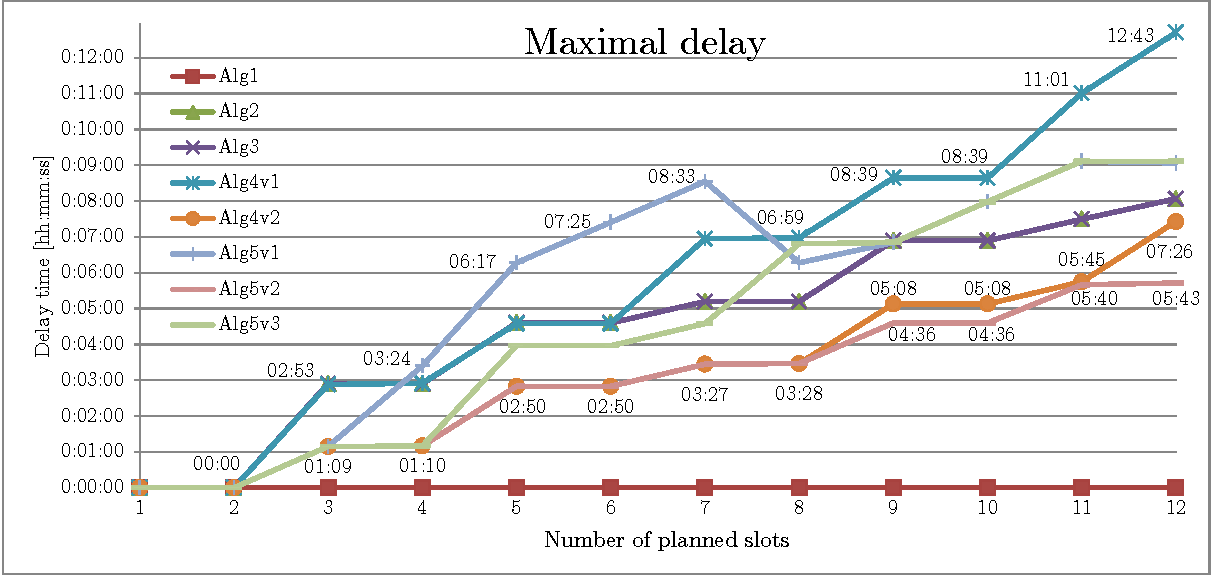
\includegraphics[width=\textwidth]{graphs/1rwy-alternating-maximal-delay.pdf}
    \caption{Graph of maximal delay for plans created with different algorithms on single runway}
    \label{graph:1rwy-alternating-maximal-delay}
\end{figure}

Another criterion that can describe the quality of a runway plan is the maximal delay among all slots. Obviously the smaller the delay is, the better the plan is. This criterion criterion can be used to prevent the situation in which one plane would give the priority to all others and would wait until its supply of fuel is depleted. The sum of all delays can be small, but the fact that the critical delay time for one aircraft was exceeded renders such plan potentially dangerous.

Graph \ref{graph:1rwy-alternating-maximal-delay} shows the development of values of this criterion during the planning. The optimal value for the final plan is 5 minutes and 43 seconds and is achieved by {\em Algorithm~5v2}. {\em Algorithm~4v1} has the poorest performance with the value of 12:43. {\em Algorithm~5v1} optimizes the total makespan and in order to do that it can delay some slots by a significant amount of time. This can lead to high maximal delay values as shown here for plans with 4 – 7 slots. {\em Algorithm~4v2} performs very well with its result at or very near the optimal value. For the final plan the maximal delay for this algorithm is 1 minute 43 second longer than the optimal value.

\subsection{Total delay}

\begin{figure}[h]
    \centering
    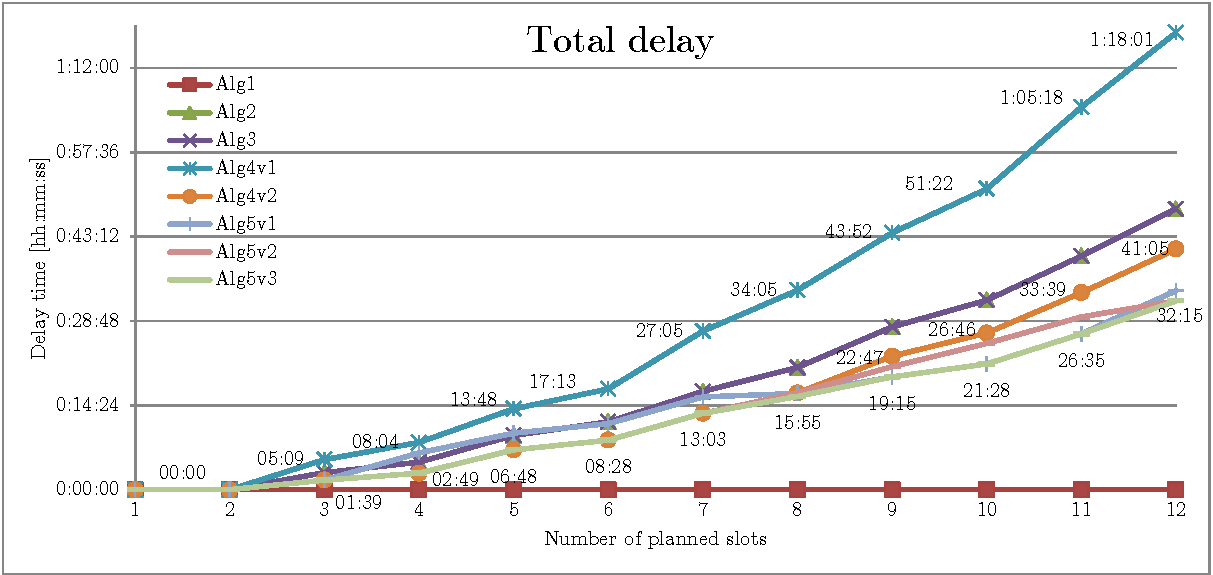
\includegraphics[width=\textwidth]{graphs/1rwy-alternating-total-delay.pdf}
    \caption{Graph of total delay for plans created with different algorithms on single runway}
    \label{graph:1rwy-alternating-total-delay}
\end{figure}

The sum of all slot delays is another way to measure runway plan's quality. It describes the total time wasted on waiting in the terminal area. It is also linked to the total amount of fuel burnt during the waiting. Both time and used amount of fuel affect the costs of the flight.

The total delay times in the progress of planning are shown in Graph \ref{graph:1rwy-alternating-total-delay}. The poorest results are again given by {\em Algorithm~4v1} with the total delay more than 2.4 times the optimum. The optimal result is produced by {\em Algorithm~5v3} (32:25 for final plan) with other two versions of the {\em Algorithm~5} very near. {\em Algorithm~4v2} performs well with the total delay at 41:05 which is less than 30\% more than the optimum. {\em Algorithm~2} and {\em Algorithm~3} still perform good and could produce usable results but are not as good as {\em Algorithm~4v2}.

\subsection{Replanned slots}

\begin{figure}[h]
    \centering
    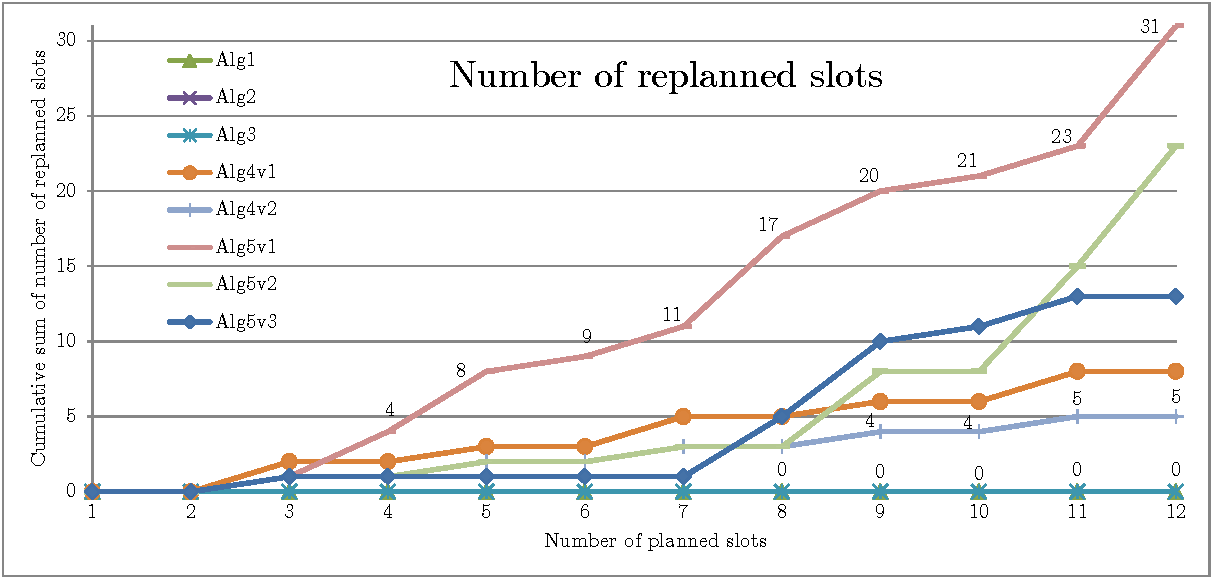
\includegraphics[width=\textwidth]{graphs/1rwy-alternating-replanned-slots.pdf}
    \caption{Graph of cumulative sum of replanned slots for plans created with different algorithms on single runway}
    \label{graph:1rwy-alternating-replanned-slots}
\end{figure}

The number of replanned slots shown in Graph \ref{graph:1rwy-alternating-replanned-slots} expresses how often the controller must interfere with the schedule of previously planned aircraft after a new one has been added to the plan. This criterion has a relation to the controllers workload, because he/she must contact each replanned aircraft and give the pilot updated instructions.

{\em Algorithm~1}, {\em Algorithm~2} and {\em Algorithm~3} place the new slots in a way that doesn't affect the previously planned and therefore don't cause the need to replan old slots. {\em Algorithm~4v2} with five replanned slots during the creation of final plan produces very good results according to the aforementioned criteria but is still undemanding of frequent replanning of old slots. All three versions of {\em Algorithm~5} have high numbers of replanned slots because the fat that they look for optimal solution causes them to change the plan significantly with each slot addition. This is especially true for {\em Algorithm~5v1} which minimizes the total makespan. Its 31 replanned slots during the creation of plan for 12 planes render it unusable for real world application.

\subsection{Conclusion}

{\em Algorithm~1} isn't intended for real-world use and it's performance is irrelevant. {\em Algorithm~2} and {\em Algorithm~3} behave identically in this scenario providing usable results in every measured aspect with the main advantage being that previously planned slots are fixed and there is no need to update the pilots instruction when new plane flies in. {\em Algorithm~4v1} performs poorly and doesn't handle the alternating weight classes well. On the other hand, similar {\em Algorithm~4v2} that adds the local optimization of delay, gives good results not too far from optimal solution with low number of slots being replanned. {\em Algorithm~5v1–3} obviously give the optimal result in the categories they are optimizing for but can have inferior results in other categories (e.g. versions 1 and 3 for maximal delay). The fact that the algorithms strive for the optimum result also means that these algorithms tend to replan previous slots often causing high workload for the controller. This and their computational complexity makes them unusable in real-world application.

\section{Real world flights on single runway}

\red{TODO}

\section{Estimation of route duration}

\red{TODO}

%\section{Comparison To Real Air Traffic}
%\section{Flight Duration}
%\section{Fuel Consumption}
%\section{Controller Workload}
%\section{Airport/Runway capacity}
%!TEX root = index.tex
\chapter{Conclusion}
\section{Future work}


%!TEX root = index.tex

%\bibliographystyle{abbrv}
%\bibliographystyle{plain}
%\bibliographystyle{psc}
%{
%JZ: 11.12.2008 Kdo chce mit v techto ukazkovych odkazech take odkaz na CSTeX:
%\def\CS{$\cal C\kern-0.1667em\lower.5ex\hbox{$\cal S$}\kern-0.075em $}
%\bibliography{bibliografie}
%}

%!TEX root = index.tex

\cleardoublepage 
\begin{thebibliography}{1}

\bibitem{growth}
ICAO.
\newblock {\em Strong Passenger Results and a Rebound for Freight Traffic in 2014.}
\newblock International Civil Aviation Organization, Montréal, 18 December 2014.
\newblock Available at: \url{http://www.icao.int/Newsroom/NewsDoc2014/COM.48.14.EN.pdf}

\bibitem{atm}
Eurocontrol.
\newblock {\em What is air traffic management} [online].
\newblock European Organisation for the Safety of Air Navigation [cited 2014-11-16].
\newblock Available at: \url{http://www.eurocontrol.int/articles/what-air-traffic-management}

\bibitem{nolan}
M.~S. Nolan.
\newblock {\em Fundamentals of air traffic control}.
\newblock Thomson--Brooks/Cole, Belmont, CA, 4th edition, 2004.

\bibitem{aim}
United States Department of Transportation, Federal Aviation Administration.
\newblock {\em Aeronautical Information Manual - Official Guide to Basic Flight Information and ATC Procedures}.
\newblock United States Department of Transportation, Federal Aviation Administration, 2014.
\newblock Available at: \url{https://www.faa.gov/air_traffic/publications/ATpubs/AIM/}.

\bibitem{doc4444}
ICAO.
\newblock {\em Doc 4444 – Air traffic management}.
\newblock International Civil Aviation Organization, Montréal, 15th edition, 2007.

\bibitem{doc8168}
ICAO.
\newblock {\em Doc 8168 – Aircraft Operations Volume I, Flight Procedures}.
\newblock International Civil Aviation Organization, Montréal, 5th edition, 2006.

\bibitem{annex11}
ICAO.
\newblock {\em Annex 11 to the Convention on International Civil Aviation: Air Traffic Services}.
\newblock International Civil Aviation Organization, 2001.

\bibitem{annex6}
ICAO.
\newblock {\em Annex 6 to the Convention on International Civil Aviation: Operation of Aircraft (Part I: International Commercial Air Transport — Aeroplanes)}.
\newblock International Civil Aviation Organization, 9th edition, 2010.

\bibitem{classes}
{\em Airspace class. in: Wikipedia: the free encyclopedia} [online].
\newblock San Francisco: Wikimedia foundation, 2001- [cited 2014-11-18].
\newblock Available at: \url{http://en.wikipedia.org/wiki/Airspace_class}

\bibitem{order7110}
United States Department of Transportation, Federal Aviation Administration.
\newblock {\em ORDER JO 7110.65U: Air Traffic Control}.
\newblock Available at: \url{http://www.faa.gov/air_traffic/publications/atpubs/ATC/index.htm}.

\bibitem{vor}
{\em VHF omnidirectional range. in: Wikipedia: the free encyclopedia} [online].
\newblock San Francisco: Wikimedia foundation, 2001- [cited 2014-11-26].
\newblock Available at: \url{http://en.wikipedia.org/wiki/VHF_omnidirectional_range}

\bibitem{agentfly-atm}
D. Šislák, P. Volf, D. Pavlíček and M. Pěchouček
\newblock {\em AGENTFLY: Multi-Agent Simulation of Air-Traffic Management}.
\newblock 2012.

\bibitem{agentfly-enroute}
D. Šišlák, P. Volf, M. Pěchouček, Ch. T. Cannon, D. N. Nguyen and W. C. Regli
\newblock {\em Multi-Agent Simulation of En-Route Human Air-Traffic Controller}.
\newblock 2012.

\bibitem{bada}
Eurocontrol.
\newblock {\em Base of Aircraft Data (BADA)} [online].
\newblock European Organisation for the Safety of Air Navigation [cited 2014-11-30].
\newblock Available at: \url{https://www.eurocontrol.int/services/bada}

\bibitem{bab}
J. Clausen.
\newblock {\em Branch and Bound Algorithms – Principles and Examples}.
\newblock 1999.
\newblock Available at: \url{http://www.imada.sdu.dk/Employees/jbj/heuristikker/TSPtext.pdf}

\bibitem{runway-throughput}
Tamas Kolos-Lakatos.
\newblock {\em The Influence of Runway Occupancy Time and Wake Vortex Separation Requirements on Runway Throughput}.
\newblock MIT International Center for Air Transportation (ICAT) Department of Aeronautics \& Astronautics Massachusetts Institute of Technology, 2013.

\bibitem{atlanta}
{\em Hartsfield–Jackson Atlanta International Airport. in: Wikipedia: the free encyclopedia} [online].
\newblock San Francisco: Wikimedia foundation, 2001- [cited 2014-12-03]. \\
\newblock Available~at: \url{http://en.wikipedia.org/wiki/Hartsfield\%E2\%80\%93Jackson_Atlanta_International_Airport}

\bibitem{atlanta-diagram}
United States Department of Transportation, Federal Aviation Administration.
\newblock {\em Airport Diagram – Hartsfield-Jackson Atlanta Intl. (ATL).}
\newblock 11 December 2014.
\newblock Available~at: \url{http://aeronav.faa.gov/d-tpp/1413/00026ad.pdf}

\bibitem{atlanta-tma}
United States Department of Transportation, Federal Aviation Administration.
\newblock {\em Document 2013-00287 – Amendment to Class B Airspace; Atlanta, GA.}
\newblock 9 January 2013.
\newblock Available~at: \url{https://www.federalregister.gov/articles/2013/01/09/2013-00287/amendment-to-class-b-airspace-atlanta-ga}

\bibitem{scheduling}
Susanne Albers. 
\newblock {\em Online scheduling.}
\newblock In Introduction to Scheduling, edited by Yves Robert and Frederic Vivien. 
\newblock Chapman and Hall/CRC Press, 57-84, 2009.
\newblock Available~at: \url{http://www14.in.tum.de/personen/albers/papers/sched_chapter.pdf}

\end{thebibliography}
\newpage
%!TEX root = index.tex

\appendix

\chapter{Testování zaplnění stránky a odsazení odstavců}
\textbf{\large Tato příloha nebude součástí vaší práce. 
Slouží pouze jako příklad formátování textu.}

\section*{}
Určitě existuje nějaká pěkná latinská věta, která se k tomuhle testování používá, ale co mají dělat ti, kteří se nikdy latinsky neučili? Určitě existuje nějaká pěkná latinská věta, která se k tomuhle testování používá, ale co mají dělat ti, kteří se nikdy latinsky neučili? Určitě existuje nějaká pěkná latinská věta, která se k tomuhle testování používá, ale co mají dělat ti, kteří se nikdy latinsky neučili?

Určitě existuje nějaká pěkná latinská věta, která se k tomuhle testování používá, ale co mají dělat ti, kteří se nikdy latinsky neučili? Určitě existuje nějaká pěkná latinská věta, která se k tomuhle testování používá, ale co mají dělat ti, kteří se nikdy latinsky neučili? Určitě existuje nějaká pěkná latinská věta, která se k tomuhle testování používá, ale co mají dělat ti, kteří se nikdy latinsky neučili?

Určitě existuje nějaká pěkná latinská věta, která se k tomuhle testování používá, ale co mají dělat ti, kteří se nikdy latinsky neučili? Určitě existuje nějaká pěkná latinská věta, která se k tomuhle testování používá, ale co mají dělat ti, kteří se nikdy latinsky neučili? Určitě existuje nějaká pěkná latinská věta, která se k tomuhle testování používá, ale co mají dělat ti, kteří se nikdy latinsky neučili?

Určitě existuje nějaká pěkná latinská věta, která se k tomuhle testování používá, ale co mají dělat ti, kteří se nikdy latinsky neučili? Určitě existuje nějaká pěkná latinská věta, která se k tomuhle testování používá, ale co mají dělat ti, kteří se nikdy latinsky neučili? Určitě existuje nějaká pěkná latinská věta, která se k tomuhle testování používá, ale co mají dělat ti, kteří se nikdy latinsky neučili? Určitě existuje nějaká pěkná latinská věta, která se k tomuhle testování používá, ale co mají dělat ti, kteří se nikdy latinsky neučili? Určitě existuje nějaká pěkná latinská věta, která se k tomuhle testování používá, ale co mají dělat ti, kteří se nikdy latinsky neučili? Určitě existuje nějaká pěkná latinská věta, která se k tomuhle testování používá, ale co mají dělat ti, kteří se nikdy latinsky neučili?

Určitě existuje nějaká pěkná latinská věta, která se k tomuhle testování používá, ale co mají dělat ti, kteří se nikdy latinsky neučili? Určitě existuje nějaká pěkná latinská věta, která se k tomuhle testování používá, ale co mají dělat ti, kteří se nikdy latinsky neučili?

Určitě existuje nějaká pěkná latinská věta, která se k tomuhle testování používá, ale co mají dělat ti, kteří se nikdy latinsky neučili? Určitě existuje nějaká pěkná latinská věta, která se k tomuhle testování používá, ale co mají dělat ti, kteří se nikdy latinsky neučili? Určitě existuje nějaká pěkná latinská věta, která se k tomuhle testování používá, ale co mají dělat ti, kteří se nikdy latinsky neučili? Určitě existuje nějaká pěkná latinská věta, která se k tomuhle testování používá, ale co mají dělat ti, kteří se nikdy latinsky neučili? Určitě existuje nějaká pěkná latinská věta, která se k tomuhle testování používá, ale co mají dělat ti, kteří se nikdy latinsky neučili?

Určitě existuje nějaká pěkná latinská věta, která se k tomuhle testování používá, ale co mají dělat ti, kteří se nikdy latinsky neučili? Určitě existuje nějaká pěkná latinská věta, která se k tomuhle testování používá, ale co mají dělat ti, kteří se nikdy latinsky neučili? Určitě existuje nějaká pěkná latinská věta, která se k tomuhle testování používá, ale co mají dělat ti, kteří se nikdy latinsky neučili? Určitě existuje nějaká pěkná latinská věta, která se k tomuhle testování používá, ale co mají dělat ti, kteří se nikdy latinsky neučili? Určitě existuje nějaká pěkná latinská věta, která se k tomuhle testování používá, ale co mají dělat ti, kteří se nikdy latinsky neučili?

Určitě existuje nějaká pěkná latinská věta, která se k tomuhle testování používá, ale co mají dělat ti, kteří se nikdy latinsky neučili? Určitě existuje nějaká pěkná latinská věta, která se k tomuhle testování používá, ale co mají dělat ti, kteří se nikdy latinsky neučili? Určitě existuje nějaká pěkná latinská věta, která se k tomuhle testování používá, ale co mají dělat ti, kteří se nikdy latinsky neučili? Určitě existuje nějaká pěkná latinská věta, která se k tomuhle testování používá, ale co mají dělat ti, kteří se nikdy latinsky neučili? Určitě existuje nějaká pěkná latinská věta, která se k tomuhle testování používá, ale co mají dělat ti, kteří se nikdy latinsky neučili?

Určitě existuje nějaká pěkná latinská věta, která se k tomuhle testování používá, ale co mají dělat ti, kteří se nikdy latinsky neučili? Určitě existuje nějaká pěkná latinská věta, která se k tomuhle testování používá, ale co mají dělat ti, kteří se nikdy latinsky neučili? Určitě existuje nějaká pěkná latinská věta, která se k tomuhle testování používá, ale co mají dělat ti, kteří se nikdy latinsky neučili? Určitě existuje nějaká pěkná latinská věta, která se k tomuhle testování používá, ale co mají dělat ti, kteří se nikdy latinsky neučili? Určitě existuje nějaká pěkná latinská věta, která se k tomuhle testování používá, ale co mají dělat ti, kteří se nikdy latinsky neučili?

Určitě existuje nějaká pěkná latinská věta, která se k tomuhle testování používá, ale co mají dělat ti, kteří se nikdy latinsky neučili? Určitě existuje nějaká pěkná latinská věta, která se k tomuhle testování používá, ale co mají dělat ti, kteří se nikdy latinsky neučili? Určitě existuje nějaká pěkná latinská věta, která se k tomuhle testování používá, ale co mají dělat ti, kteří se nikdy latinsky neučili? Určitě existuje nějaká pěkná latinská věta, která se k tomuhle testování používá, ale co mají dělat ti, kteří se nikdy latinsky neučili? Určitě existuje nějaká pěkná latinská věta, která se k tomuhle testování používá, ale co mají dělat ti, kteří se nikdy latinsky neučili?

Určitě existuje nějaká pěkná latinská věta, která se k tomuhle testování používá, ale co mají dělat ti, kteří se nikdy latinsky neučili? Určitě existuje nějaká pěkná latinská věta, která se k tomuhle testování používá, ale co mají dělat ti, kteří se nikdy latinsky neučili? Určitě existuje nějaká pěkná latinská věta, která se k tomuhle testování používá, ale co mají dělat ti, kteří se nikdy latinsky neučili? Určitě existuje nějaká pěkná latinská věta, která se k tomuhle testování používá, ale co mají dělat ti, kteří se nikdy latinsky neučili? Určitě existuje nějaká pěkná latinská věta, která se k tomuhle testování používá, ale co mají dělat ti, kteří se nikdy latinsky neučili?

Určitě existuje nějaká pěkná latinská věta, která se k tomuhle testování používá, ale co mají dělat ti, kteří se nikdy latinsky neučili? Určitě existuje nějaká pěkná latinská věta, která se k tomuhle testování používá, ale co mají dělat ti, kteří se nikdy latinsky neučili? Určitě existuje nějaká pěkná latinská věta, která se k tomuhle testování používá, ale co mají dělat ti, kteří se nikdy latinsky neučili? Určitě existuje nějaká pěkná latinská věta, která se k tomuhle testování používá, ale co mají dělat ti, kteří se nikdy latinsky neučili? Určitě existuje nějaká pěkná latinská věta, která se k tomuhle testování používá, ale co mají dělat ti, kteří se nikdy latinsky neučili?

Určitě existuje nějaká pěkná latinská věta, která se k tomuhle testování používá, ale co mají dělat ti, kteří se nikdy latinsky neučili? Určitě existuje nějaká pěkná latinská věta, která se k tomuhle testování používá, ale co mají dělat ti, kteří se nikdy latinsky neučili? Určitě existuje nějaká pěkná latinská věta, která se k tomuhle testování používá, ale co mají dělat ti, kteří se nikdy latinsky neučili? Určitě existuje nějaká pěkná latinská věta, která se k tomuhle testování používá, ale co mají dělat ti, kteří se nikdy latinsky neučili? Určitě existuje nějaká pěkná latinská věta, která se k tomuhle testování používá, ale co mají dělat ti, kteří se nikdy latinsky neučili?

Určitě existuje nějaká pěkná latinská věta, která se k tomuhle testování používá, ale co mají dělat ti, kteří se nikdy latinsky neučili? Určitě existuje nějaká pěkná latinská věta, která se k tomuhle testování používá, ale co mají dělat ti, kteří se nikdy latinsky neučili? Určitě existuje nějaká pěkná latinská věta, která se k tomuhle testování používá, ale co mají dělat ti, kteří se nikdy latinsky neučili? Určitě existuje nějaká pěkná latinská věta, která se k tomuhle testování používá, ale co mají dělat ti, kteří se nikdy latinsky neučili? Určitě existuje nějaká pěkná latinská věta, která se k tomuhle testování používá, ale co mají dělat ti, kteří se nikdy latinsky neučili?

Určitě existuje nějaká pěkná latinská věta, která se k tomuhle testování používá, ale co mají dělat ti, kteří se nikdy latinsky neučili? Určitě existuje nějaká pěkná latinská věta, která se k tomuhle testování používá, ale co mají dělat ti, kteří se nikdy latinsky neučili? Určitě existuje nějaká pěkná latinská věta, která se k tomuhle testování používá, ale co mají dělat ti, kteří se nikdy latinsky neučili? Určitě existuje nějaká pěkná latinská věta, která se k tomuhle testování používá, ale co mají dělat ti, kteří se nikdy latinsky neučili? Určitě existuje nějaká pěkná latinská věta, která se k tomuhle testování používá, ale co mají dělat ti, kteří se nikdy latinsky neučili?

Určitě existuje nějaká pěkná latinská věta, která se k tomuhle testování používá, ale co mají dělat ti, kteří se nikdy latinsky neučili? Určitě existuje nějaká pěkná latinská věta, která se k tomuhle testování používá, ale co mají dělat ti, kteří se nikdy latinsky neučili? Určitě existuje nějaká pěkná latinská věta, která se k tomuhle testování používá, ale co mají dělat ti, kteří se nikdy latinsky neučili? Určitě existuje nějaká pěkná latinská věta, která se k tomuhle testování používá, ale co mají dělat ti, kteří se nikdy latinsky neučili? Určitě existuje nějaká pěkná latinská věta, která se k tomuhle testování používá, ale co mají dělat ti, kteří se nikdy latinsky neučili?

Určitě existuje nějaká pěkná latinská věta, která se k tomuhle testování používá, ale co mají dělat ti, kteří se nikdy latinsky neučili? Určitě existuje nějaká pěkná latinská věta, která se k tomuhle testování používá, ale co mají dělat ti, kteří se nikdy latinsky neučili? Určitě existuje nějaká pěkná latinská věta, která se k tomuhle testování používá, ale co mají dělat ti, kteří se nikdy latinsky neučili? Určitě existuje nějaká pěkná latinská věta, která se k tomuhle testování používá, ale co mají dělat ti, kteří se nikdy latinsky neučili? Určitě existuje nějaká pěkná latinská věta, která se k tomuhle testování používá, ale co mají dělat ti, kteří se nikdy latinsky neučili?

Určitě existuje nějaká pěkná latinská věta, která se k tomuhle testování používá, ale co mají dělat ti, kteří se nikdy latinsky neučili? Určitě existuje nějaká pěkná latinská věta, která se k tomuhle testování používá, ale co mají dělat ti, kteří se nikdy latinsky neučili? Určitě existuje nějaká pěkná latinská věta, která se k tomuhle testování používá, ale co mají dělat ti, kteří se nikdy latinsky neučili? Určitě existuje nějaká pěkná latinská věta, která se k tomuhle testování používá, ale co mají dělat ti, kteří se nikdy latinsky neučili? Určitě existuje nějaká pěkná latinská věta, která se k tomuhle testování používá, ale co mají dělat ti, kteří se nikdy latinsky neučili?

Určitě existuje nějaká pěkná latinská věta, která se k tomuhle testování používá, ale co mají dělat ti, kteří se nikdy latinsky neučili? Určitě existuje nějaká pěkná latinská věta, která se k tomuhle testování používá, ale co mají dělat ti, kteří se nikdy latinsky neučili? Určitě existuje nějaká pěkná latinská věta, která se k tomuhle testování používá, ale co mají dělat ti, kteří se nikdy latinsky neučili? Určitě existuje nějaká pěkná latinská věta, která se k tomuhle testování používá, ale co mají dělat ti, kteří se nikdy latinsky neučili? Určitě existuje nějaká pěkná latinská věta, která se k tomuhle testování používá, ale co mají dělat ti, kteří se nikdy latinsky neučili?

Určitě existuje nějaká pěkná latinská věta, která se k tomuhle testování používá, ale co mají dělat ti, kteří se nikdy latinsky neučili? Určitě existuje nějaká pěkná latinská věta, která se k tomuhle testování používá, ale co mají dělat ti, kteří se nikdy latinsky neučili? Určitě existuje nějaká pěkná latinská věta, která se k tomuhle testování používá, ale co mají dělat ti, kteří se nikdy latinsky neučili? Určitě existuje nějaká pěkná latinská věta, která se k tomuhle testování používá, ale co mají dělat ti, kteří se nikdy latinsky neučili? Určitě existuje nějaká pěkná latinská věta, která se k tomuhle testování používá, ale co mají dělat ti, kteří se nikdy latinsky neučili?

%*****************************************************************************
\chapter{Pokyny a návody k formátování textu práce}
\textbf{\large Tato příloha samozřejmě nebude součástí vaší práce. Slouží pouze jako příklad formátování textu.}

Používat se dají všechny příkazy systému \LaTeX. Existuje velké množství volně přístupné dokumentace, tutoriálů, příruček a dalších materiálů v elektronické podobě. Výchozím bodem, kromě Googlu, může být stránka CSTUG (Czech Tech Users Group) \cite{CSTUG}. Tam najdete odkazy na další materiály.  Vetšinou dostačující a přehledně organizovanou elektronikou dokumentaci najdete například na \cite{latexdocweb} nebo \cite{latexwiki}.

Existují i různé nadstavby nad systémy \TeX{} a \LaTeX, které výrazně usnadní psaní textu zejména začátečníkům. Velmi rozšířený v Linuxovém prostředí je systém Kile.


\section{Vkládání obrázků}
Obrázky se umísťují do plovoucího prostředí \verb|figure|. Každý obrázek by měl obsahovat \textbf{název} (\verb|\caption|) a \textbf{návěští} (\verb|\label|). Použití příkazu pro vložení obrázku \\\verb|\includegraphics| je podmíněno aktivací (načtením) balíku graphicx příkazem\\ \verb|\usepackage{graphicx}|.

Budete-li zdrojový text zpracovávat pomocí programu \verb|pdflatex|, očekávají se obrázky s příponou \verb|*.pdf|\footnote{pdflatex umí také formáty PNG a JPG.}, použijete-li k formátování \verb|latex|, očekávají se obrázky s příponou \verb|*.eps|.\footnote{Vzájemnou konverzi mezi snad všemi typy obrazku včetně změn vekostí a dalších vymožeností vám může zajistit balík ImageMagic  (http://www.imagemagick.org/script/index.php). Je dostupný pod Linuxem, Mac OS i MS Windows. Důležité jsou zejména příkazy convert a identify.}

\begin{figure}[ht]
\begin{center}

\includegraphics[width=5cm]{figures/LogoCVUT}
\caption{Popiska obrázku}
\label{fig:logo}
\end{center}
\end{figure}

Příklad vložení obrázku:
\begin{verbatim}
\begin{figure}[h]
\begin{center}

\includegraphics[width=5cm]{figures/LogoCVUT}
\caption{Popiska obrazku}
\label{fig:logo}
\end{center}
\end{figure}
\end{verbatim}

\section{Kreslení obrázků}
Zřejmě každý z vás má nějaký oblíbený nástroj pro tvorbu obrázků. Jde jen o to, abyste dokázali obrázek uložit v požadovaném formátu nebo jej do něj konvertovat (viz předchozí kapitola). Je zřejmě vhodné kreslit obrázky vektorově. Celkem oblíbený, na ovládání celkem jednoduchý a přitom dostatečně mocný je například program Inkscape.

Zde stojí za to upozornit na kreslící programe Ipe \cite{ipe}, který dokáže do obrázku vkládat komentáře přímo v latexovském formátu (vzroce, stejné fonty atd.). Podobné věci umí na Linuxové platformě nástroj Xfig. 

Za pozornost ještě stojí schopnost editoru Ipe importovat obrázek (jpg nebo bitmap) a krelit do něj latexovské popisky a komentáře. Výsledek pak umí exportovat přímo do pdf.

\section{Tabulky}
Existuje více způsobů, jak sázet tabulky. Například je možno použít prostředí \verb|table|, které je velmi podobné prostředí \verb|figure|. 

\begin{table}
\begin{center}
\begin{tabular}{|c|l|l|}
\hline
\textbf{DTD} & \textbf{construction} & \textbf{elimination} \\
\hline
$\mid$ & \verb+in1|A|B a:sum A B+ & \verb+case([_:A]a)([_:B]a)ab:A+\\
&\verb+in1|A|B b:sum A B+ & \verb+case([_:A]b)([_:B]b)ba:B+\\
\hline
$+$&\verb+do_reg:A -> reg A+&\verb+undo_reg:reg A -> A+\\
\hline
$*,?$& the same like $\mid$ and $+$ & the same like $\mid$ and $+$\\
& with \verb+emtpy_el:empty+ & with \verb+emtpy_el:empty+\\
\hline
R(a,b) & \verb+make_R:A->B->R+ & \verb+a: R -> A+\\
 & & \verb+b: R -> B+\\
\hline
\end{tabular}
\end{center}
\caption{Ukázka tabulky}
\label{tab:tab1}
\end{table}

Zdrojový text tabulky \ref{tab:tab1} vypadá takto:
\begin{verbatim}
\begin{table}
\begin{center}
\begin{tabular}{|c|l|l|}
\hline
\textbf{DTD} & \textbf{construction} & \textbf{elimination} \\
\hline
$\mid$ & \verb+in1|A|B a:sum A B+ & \verb+case([_:A]a)([_:B]a)ab:A+\\
&\verb+in1|A|B b:sum A B+ & \verb+case([_:A]b)([_:B]b)ba:B+\\
\hline
$+$&\verb+do_reg:A -> reg A+&\verb+undo_reg:reg A -> A+\\
\hline
$*,?$& the same like $\mid$ and $+$ & the same like $\mid$ and $+$\\
& with \verb+emtpy_el:empty+ & with \verb+emtpy_el:empty+\\
\hline
R(a,b) & \verb+make_R:A->B->R+ & \verb+a: R -> A+\\
 & & \verb+b: R -> B+\\
\hline
\end{tabular}
\end{center}
\caption{Ukázka tabulky}
\label{tab:tab1}
\end{table}
\begin{table}
\end{verbatim}

\section{Odkazy v textu}
\subsection{Odkazy na literaturu}
Jsou realizovány příkazem \verb|\cite{odkaz}|. 

Seznam literatury je dobré zapsat do samostatného souboru a ten pak zpracovat programem bibtex (viz soubor \verb|reference.bib|). Zdrojový soubor pro \verb|bibtex| vypadá například takto:
\begin{verbatim}
@Article{Chen01,
  author  = "Yong-Sheng Chen and Yi-Ping Hung and Chiou-Shann Fuh",
  title   = "Fast Block Matching Algorithm Based on 
             the Winner-Update Strategy",
  journal = "IEEE Transactions On Image Processing",
  pages   = "1212--1222",
  volume  =  10,
  number  =   8,
  year    = 2001,
}

@Misc{latexdocweb,
  author  = "",
  title   = "{\LaTeX} --- online manuál",
  note    = "\verb|http://www.cstug.cz/latex/lm/frames.html|",
  year    = "",
}
...
\end{verbatim}

%11.12.2008, 3.5.2009
\textbf{Pozor:} Sazba názvů odkazů je dána Bib\TeX{} stylem\\ (\verb|\bibliographystyle{abbrv}|). 
%Budete-li používat české prostředí (\verb|\usepackage[czech]{babel}|), 
Bib\TeX{} tedy obvykle vysází velké pouze počáteční písmeno z názvu zdroje, 
ostatní písmena zůstanou malá bez ohledu na to, jak je napíšete. 
Přesněji řečeno, styl může zvolit pro každý typ publikace jiné konverze. 
Pro časopisecké články třeba výše uvedené, jiné pro monografie (u nich často bývá 
naopak velikost písmen zachována).

Pokud chcete Bib\TeX u napovědět, která písmena nechat bez konverzí 
(viz \texttt{title = "\{$\backslash$LaTeX\} -{}-{}- online manuál"} 
v~předchozím příkladu), je nutné příslušné písmeno (zde celé makro) uzavřít 
do složených závorek. Pro přehlednost je proto vhodné celé parametry 
uzavírat do uvozovek (\texttt{author = "\dots"}), nikoliv do složených závorek.

Odkazy na literaturu ve zdrojovém textu se pak zapisují:
\begin{verbatim}
Podívejte se na \cite{Chen01}, 
další detaily najdete na \cite{latexdocweb}
\end{verbatim}

Vazbu mezi soubory \verb|*.tex| a \verb|*.bib| zajistíte příkazem 
\verb|\bibliography{}| v souboru \verb|*.tex|.  V našem případě tedy zdrojový 
dokument \verb|thesis.tex| obsahuje příkaz\\
\verb|\bibliography{reference}|.

Zpracování zdrojového textu s odkazy se provede postupným voláním programů\\
\verb|pdflatex <soubor>| (případně \verb|latex <soubor>|), \verb|bibtex <soubor>| 
a opět\\ \verb|pdflatex <soubor>|.\footnote{První volání \texttt{pdflatex} 
vytvoří soubor s~koncovkou \texttt{*.aux}, který je vstupem pro program 
\texttt{bibtex}, pak je potřeba znovu zavolat program \texttt{pdflatex} 
(\texttt{latex}), který tentokrát zpracuje soubory s příponami \texttt{.aux} a 
\texttt{.tex}. 
Informaci o případných nevyřešených odkazech (cross-reference) vidíte přímo při 
zpracovávání zdrojového souboru příkazem \texttt{pdflatex}. Program \texttt{pdflatex} 
(\texttt{latex}) lze volat vícekrát, pokud stále vidíte nevyřešené závislosti.}


Níže uvedený příklad je převzat z dříve existujících pokynů studentům, kteří 
dělají svou diplomovou nebo bakalářskou práci v~Grafické skupině.\footnote{Několikrát 
jsem byl upozorněn, že web s těmito pokyny byl zrušen, proto jej zde přímo necituji. 
Nicméně příklad sám o sobě dokumentuje obecně přijímaný konsensus ohledně citací 
v~bakalářských a diplomových pracích na KP.} Zde se praví:
\begin{small}
\begin{verbatim}
...
j) Seznam literatury a dalších použitých pramenů, odkazy na WWW stránky, ...
 Pozor na to, že na veškeré uvedené prameny se musíte v textu práce 
 odkazovat -- [1]. 
Pramen, na který neodkazujete, vypadá, že jste ho vlastně nepotřebovali 
a je uveden jen do počtu. Příklad citace knihy [1], článku v časopise [2], 
stati ve sborníku [3] a html odkazu [4]: 
[1] J. Žára, B. Beneš;, and P. Felkel. 
     Moderní počítačová grafika. Computer Press s.r.o, Brno, 1 edition, 1998. 
     (in Czech). 
[2] P. Slavík. Grammars and Rewriting Systems as Models for Graphical User 
     Interfaces. Cognitive Systems, 4(4--3):381--399, 1997. 
[3] M. Haindl, Š. Kment, and P. Slavík. Virtual Information Systems. 
     In WSCG'2000 -- Short communication papers, pages 22--27, Pilsen, 2000. 
     University of West Bohemia. 
[4] Knihovna grafické skupiny katedry počítačů: 
     http://www.cgg.cvut.cz/Bib/library/ 
\end{verbatim}
\end{small}
\ldots{} abychom výše citované odkazy skutečně našli v (automaticky generovaném) seznamu literatury tohoto textu, musíme je nyní alespoň jednou citovat: Kniha \cite{kniha}, článek v~časopisu \cite{clanek}, příspěvek na konferenci \cite{sbornik}, www odkaz \cite{www}.

\subsection{Odkazy na obrázky, tabulky a kapitoly}
\begin{itemize}
\item Označení místa v textu, na které chcete později čtenáře práce odkázat, se provede příkazem \verb|\label{navesti}|. Lze použít v prostředích \verb|figure| a  \verb|table|, ale též za názvem kapitoly nebo podkapitoly.
\item Na návěští se odkážeme příkazem \verb|\ref{navesti}| nebo \verb|\pageref{navesti}|.
\end{itemize}

\section{Rovnice, centrovaná, číslovaná matematika}
Jednoduchý matematický výraz zapsaný přímo do textu se vysází pomocí prostředí \verb|math|, resp. zkrácený zápis pomocí uzavření textu rovnice mezi znaky \verb|$|.

Kód \verb|$ S = \pi * r^2 $| bude vysázen takto: $ S = \pi * r^2 $.

Pokud chcete nečíslované rovnice, ale umístěné centrovaně na samostatné řádky, pak lze použít prostředí \verb|displaymath|, resp. zkrácený zápis pomocí uzavření textu rovnice mezi znaky \verb|$$|. Zdrojový kód: 
\begin{verb}
|$$ S = \pi * r^2 $$|
\end{verb}
bude pak vysázen takto:
$$ S = \pi * r^2 $$

Chcete-li mít rovnice číslované, je třeba použít prostředí \verb|eqation|. Kód:
\begin{verbatim}
\begin{equation}
  S = \pi * r^2
\end{equation}

\begin{equation}
  V = \pi * r^3
\end{equation}
\end{verbatim}
je potom vysázen takto:
\begin{equation}
  S = \pi * r^2
\end{equation}

\begin{equation}
  V = \pi * r^3
\end{equation}

\section{Kódy programu}
Chceme-li vysázet například část zdrojového kódu programu (bez formátování), hodí se prostředí \verb|verbatim|: 
\begin{verbatim}
         (* nickname2 *)
Lego> Refine in1
             (do_reg (nickname1 h));
Refine by  in1 (do_reg (nickname1 h))
   ?4 : pcdata
   ?5 : pcdata
          (* surname2 *)
Lego> Refine surname1 h;
Refine by  surname1 h
   ?5 : pcdata
          (* email2 *)
Lego> Refine undo_reg (email1 h);
Refine by  undo_reg (email1 h)
*** QED ***
\end{verbatim}

\section{Další poznámky}
\subsection{České uvozovky}
V souboru \verb|k336_thesis_macros.tex| je příkaz \verb|\uv{}| pro sázení českých uvozovek. \uv{Text uzavřený do českých uvozovek.}

% JZ: 3.5.2009 \chapter z book zajistí automaticky
%\subsection{Začátky kapitol na liché stránky}
%Ve výsledném textu je dobré, když každá kapitola začíná na liché stránce. Tedy použijte:
%\begin{verbatim}
%  \cleardoublepage\include{1_uvod}
%  \cleardoublepage\include{2_teorie}
%   atd.\ldots{}
%\end{verbatim}

%*****************************************************************************
%!TEX root = index.tex
\chapter{List of Used Abbreviations}

\begin{description}
\item[ATM] Air Traffic Management
\item[ATC] Air Traffic Control
\item[ATFM] Air Traffic Flow Management
\item[AIS] Aeronautical Information Services
\item[FP] Flight Plan
\item[GPS] Global Positioning System
\item[SID] Standard Instrument Departure
\item[STAR] Standard Terminal Arrival Route
\item[ACC] Area Control Service
\item[APP] Approach Control Service
\item[TWR] Aerodrome Control Service
\item[CTA] Control Area
\item[CTR] Control Zone
\item[TMA] Terminal Control Area
\item[IFR] Instrument flight rules
\item[VFR] visual flight rules

% \item[NM] Nautical mile = 1.852 km
% \item[NDB] Non Directional Beacon - nesměrový radiomaják
% \item[VOR] VHF Omnidirectional Radio Range - všesměrový radiomaják
% \item[ASM] Airspace Management
% \item[ETA] estimated time of arrival
% \item[EAT] Expected Approach Time
\end{description}

%*****************************************************************************
\chapter{UML diagramy}
\textbf{\large Tato příloha není povinná a zřejmě se neobjeví v každé práci. Máte-li ale větší množství podobných diagramů popisujících systém, není nutné všechny umísťovat do hlavního textu, zvláště pokud by to snižovalo jeho čitelnost.}

%*****************************************************************************
\chapter{Instalační a uživatelská příručka}
\textbf{\large Tato příloha velmi žádoucí zejména u softwarových implementačních prací.}

%*****************************************************************************
\chapter{Obsah přiloženého CD}
\textbf{\large Tato příloha je povinná pro každou práci. Každá práce musí totiž obsahovat přiložené CD. Viz dále.}

Může vypadat například takto. Váš seznam samozřejmě bude odpovídat typu vaší práce. (viz \cite{infodp}):

\begin{figure}[h]
\begin{center}
\includegraphics[width=14cm]{figures/seznamcd}
\caption{Seznam přiloženého CD --- příklad}
\label{fig:seznamcd}
\end{center}
\end{figure}

Na GNU/Linuxu si strukturu přiloženého CD můžete snadno vyrobit příkazem:\\ 
\verb|$ tree . >tree.txt|\\
Ve vzniklém souboru pak stačí pouze doplnit komentáře.

Z \textbf{README.TXT} (případne index.html apod.)  musí být rovněž zřejmé, jak programy instalovat, spouštět a jaké požadavky mají tyto programy na hardware.

Adresář \textbf{text}  musí obsahovat soubor s vlastním textem práce v PDF nebo PS formátu, který bude později použit pro prezentaci diplomové práce na WWW.



\end{document}

